\documentclass[a4paper,12pt]{report}
\usepackage[portuguese]{babel}
\usepackage{indentfirst}
\usepackage[T1]{fontenc}
\usepackage[utf8]{inputenc}
\usepackage{csquotes}
\usepackage{array}
\usepackage[font={footnotesize,it}]{caption}
\usepackage{graphicx} 
\usepackage{float}
\usepackage{color, colortbl}
\usepackage{titlesec}
\usepackage{longtable}
\usepackage{pdfpages} 
\graphicspath{ {./supportFiles/}}
\usepackage{tabularx}
\usepackage{soul}
\usepackage[dash, dot]{dashundergaps}
\usepackage{hyphenat}
\usepackage[export]{adjustbox}

\setlength{\parskip}{\baselineskip}

%\usepackage{lmodern} 
%\usepackage[top=2.5cm, bottom=2.5cm, left=3cm, right=2.5cm]{geometry}

\usepackage{xcolor}
\usepackage{spverbatim}

\usepackage{listings}
\definecolor{codegray}{rgb}{0.5,0.5,0.5}
\lstset{commentstyle=\color{codegray},
        keywordstyle=\color{codegray},
        numberstyle=\tiny\color{codegray},
        stringstyle=\color{codegray}
		numberstyle=\scriptsize\ttfamily, 
		numbersep=10pt,
		basicstyle=\small\ttfamily,
		breakatwhitespace=false,  
		framesep=4pt,     
		breaklines=true,
	    captionpos=b,
	    keepspaces=true,
	    numbers=left,
	    showspaces=false,
	    showstringspaces=false,
	    showtabs=false,
	    tabsize=2,
	    }

\begin{document}
	
	\begin{titlepage}
		\begin{center}
		
		\begin{figure}[H]
		\begin{center}
			
\includegraphics[scale=0.45]{logo_utad_completo_preto}	
		\end{center}
		\label{fig:logoUTAD}	
		\end{figure}
		
		\vspace{3cm}
		\huge
		\textbf{FoodFinder}
		
		%\vspace{0.5cm}
		\Large
		Design e Desenvolvimento de uma Aplicação Web\\
		Etapa 2
		
		
		\vspace{2.5cm}
		\large
		David Ferreira, 68222\\
		André Mendes, 68228\\
		João Santos, 68943\\
		Diogo Mesquita, 69185\\
		
		\vspace{2.5cm}
		Licenciatura em Engenharia Informática\\
		Laboratório de Aplicações Web e Base de Dados \\
		
		\vspace{1.5cm}		
		Vila Real, novembro de 2020
		
		\end{center}
	\end{titlepage}	
	
	
	
	
	
%--------------------------------------------------------------
	
	\pagenumbering{roman}
	
	\begin{abstract}
	Atualmente, as aplicações \textit{Web} estão em todo o lado e esta é uma tendência que continua a aumentar com cada vez mais plataformas, ferramentas e informação a transitar para serviços remotos. Desta maneira, este tipo de aplicação faz, cada vez mais, parte do nosso dia-a-dia e ocupam um espaço importante na vida das organizações.
	
	Com o intuito de proceder ao \textit{design} e implementação de uma aplicação \textit{Web} que consiste, entre várias funcionalidades, num portal de restaurantes e dos seus pratos do dia, o presente documento dedica-se a efetuar o mapeamento do modelo concetual da base de dados para o modelo físico e a consequente implementação deste último utilizando a linguagem SQL. Da mesma maneira, também serão apresentadas as \textit{mockups} da aplicação \textit{web}. Este é um passo imprescindível no planeamento desta \textit{web app} de modo a garantir que a solução final responda corretamente às necessidades do sistema a construir.
	\end{abstract}	
	
	
	\newpage
	\tableofcontents
	
	\pagenumbering{arabic}
	\newpage	
	
%--------------------------------------------------------------	
\chapter{Introdução}	

	A \textit{World Wide Web} foi introduzida no inicio da década de 1990 com o intuito de tornar possível o acesso a informação de qualquer origem de uma forma simples e consistente. Assim, desde o seu surgimento, a Internet tornou-se na plataforma de escolha para um número cada vez maior de aplicações \textit{web} inovadoras e sofisticadas (Jazayeri, 2007).
	
	Efetivamente, os dados são o coração da maioria das aplicações modernas e, assim, o \textit{design} de uma base de dados, coleção organizada de informação estruturada, é a tarefa mais importante que é executada por um desenvolvedor de aplicações. Isto, pois tanto a base de dados resultante, como todas as aplicações que dela façam uso, serão baseadas e dependentes do sucesso do \textit{design}(Captain, 2015).
	
	Por outro lado, o realizar de um rascunho das \textit{web apps} com ferramentas de \textit{mockup} é uma prática comum que melhora o processo de elicitação e validação dos requisitos da aplicação. 
	
	Dessa maneira, este documento começa por apresentar o mapeamento do modelo conceptual da base de dados para o modelo relacional e, em seguida, da apresentação do código SQL para a implementação do modelo físico. Por último, ainda serão apresentadas as várias \textit{mockups} das interfaces que constituirão a aplicação em estudo.   
	
	
%--------------------------------------------------------------
\chapter{Mapeamento do Modelo Conceptual para o Modelo Relacional}

	Após a análise do diagrama entidade-relacionamento, no anexo xxxxxxx, procedemos agora ao mapeamento do mesmo para o modelo relacional. Esse mapeamento é apresentado em seguida.
	
	Na notação que foi por nós adotada, identifica-se a \underline{chave primária} com um sublinhado contínuo e a \dotuline{chave estrangeira} com um sublinhado pontuado. Esta será a notação utilizada no decorrer deste documento.

\bigskip

Utilizador (\underline{username}, email, password, nome, registo\_confirmado, \\ \dotuline{bloqueado\_id})

\hspace*{1.5cm} bloqueado\_id referencia Bloqueio.

\medskip

Bloqueio (\underline{Id}, valor, motivo)

\medskip

Restaurante (\underline{\dotuline{restaurante\_id}}, contacto\_email, contacto\_telefone, horario\_funcionamento, dia\_de\_descanso, tipo\_de\_servico, \dotuline{localizacao\_id},\\ rating, descricao)

\hspace*{1.5cm} restaurante\_id referencia Utilizador.

\hspace*{1.5cm} localizacao\_id \& codigo\_postal referencia Localizacao.

\medskip

Comentario\_Restaurante (\underline{comentario\_id}, data, \dotuline{restaurante\_id}, \\ \dotuline{cliente\_id}, descricao, corpo)

\hspace*{1.5cm} restaurante\_id referencia Restaurante.

\hspace*{1.5cm} cliente\_id referencia Cliente.

\medskip

Localizacao (\underline{localizacao\_id}, codigo\_postal, morada, localidade, gps\_latitude, gps\_longitude)

\medskip

Administrador (\underline{\dotuline{administrador\_id}})

\hspace*{1.5cm} administrador\_id referencia Utilizador.

\medskip

Cliente (\underline{\dotuline{cliente\_id}})

\hspace*{1.5cm} cliente\_id referencia Utilizador.

\medskip

Prato\_Do\_Dia (\underline{id}, descricao, tipo)

\medskip

Adicionar\_Prato\_do\_Dia (\underline{\dotuline{restaurante\_id}}, \underline{\dotuline{prato\_id}},\\ \underline{data\_prato}, preco, destacado)

\hspace*{1.5cm} restaurante\_id referencia Restaurante.

\hspace*{1.5cm} prato\_id referencia Prato\_Do\_Dia.

\medskip

Favoritar\_Restaurante (\underline{\dotuline{restaurante\_id}}, \underline{\dotuline{cliente\_id}})

\hspace*{1.5cm} restaurante\_id referencia Restaurante.

\hspace*{1.5cm} cliente\_id referencia Cliente.

\medskip

Favoritar\_Prato\_Do\_Dia (\underline{\dotuline{prato\_id}}, \underline{\dotuline{cliente\_id}})

\hspace*{1.5cm} prato\_id referencia Prato\_Do\_Dia.

\hspace*{1.5cm} cliente\_id referencia Cliente.



%--------------------------------------------------------------
\chapter{Implementação do Modelo Físico}

	No anexo A, a partir da página \pageref{anexoA}, é apresentado o código, implementado em SQL, que permite a criação das tabelas da base de dados. 
	
	Após implementação, a base de dados assumirá o aspeto que se encontra modelado no diagrama \ref{fig:diagramaModeloFisicoSQL}.


\begin{figure}[H]
	\begin{center}
	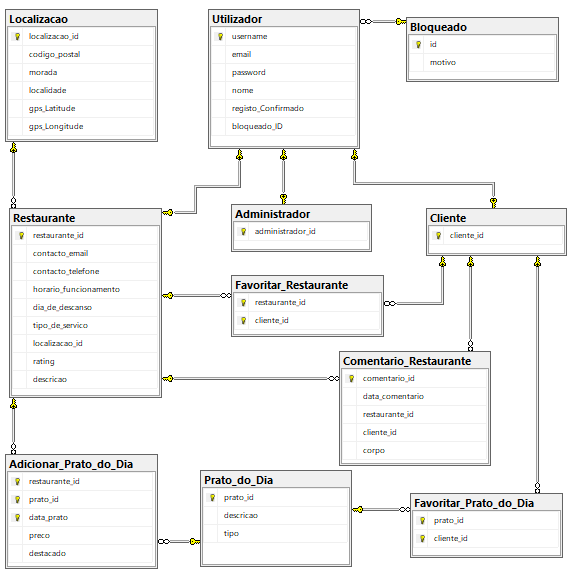
\includegraphics[scale=0.85]{diagramaModeloFisicoSQL}	
	\end{center}
	\medskip
	\caption{O diagrama representativo das tabelas da base de dados criadas com a implementação do modelo físico.}
	\label{fig:diagramaModeloFisicoSQL}	
	\end{figure}




%--------------------------------------------------------------
\chapter{\textit{Mockups} das Interfaces do Sistema}	

	Neste capítulo, são apresentadas as várias \textit{mockups} de \textit{interfaces} que constituirão o sistema.
	
	Em primeiro lugar, são apresentadas as interfaces que são comuns aos vários tipos de utilizadores do sistema (incluindo o utilizador não registado), tais como as interfaces que são específicas ao utilizador Cliente.
	
	Em seguida, são apresentadas as interfaces que dizem respeito ao utilizador restaurante. 
	
	Por último, encontram-se as interfaces especificas às funcionalidades de um administrador.	
	
\section{Interfaces Gerais e Específicas ao Cliente}
	
	\begin{figure}[H]
	\begin{center}
	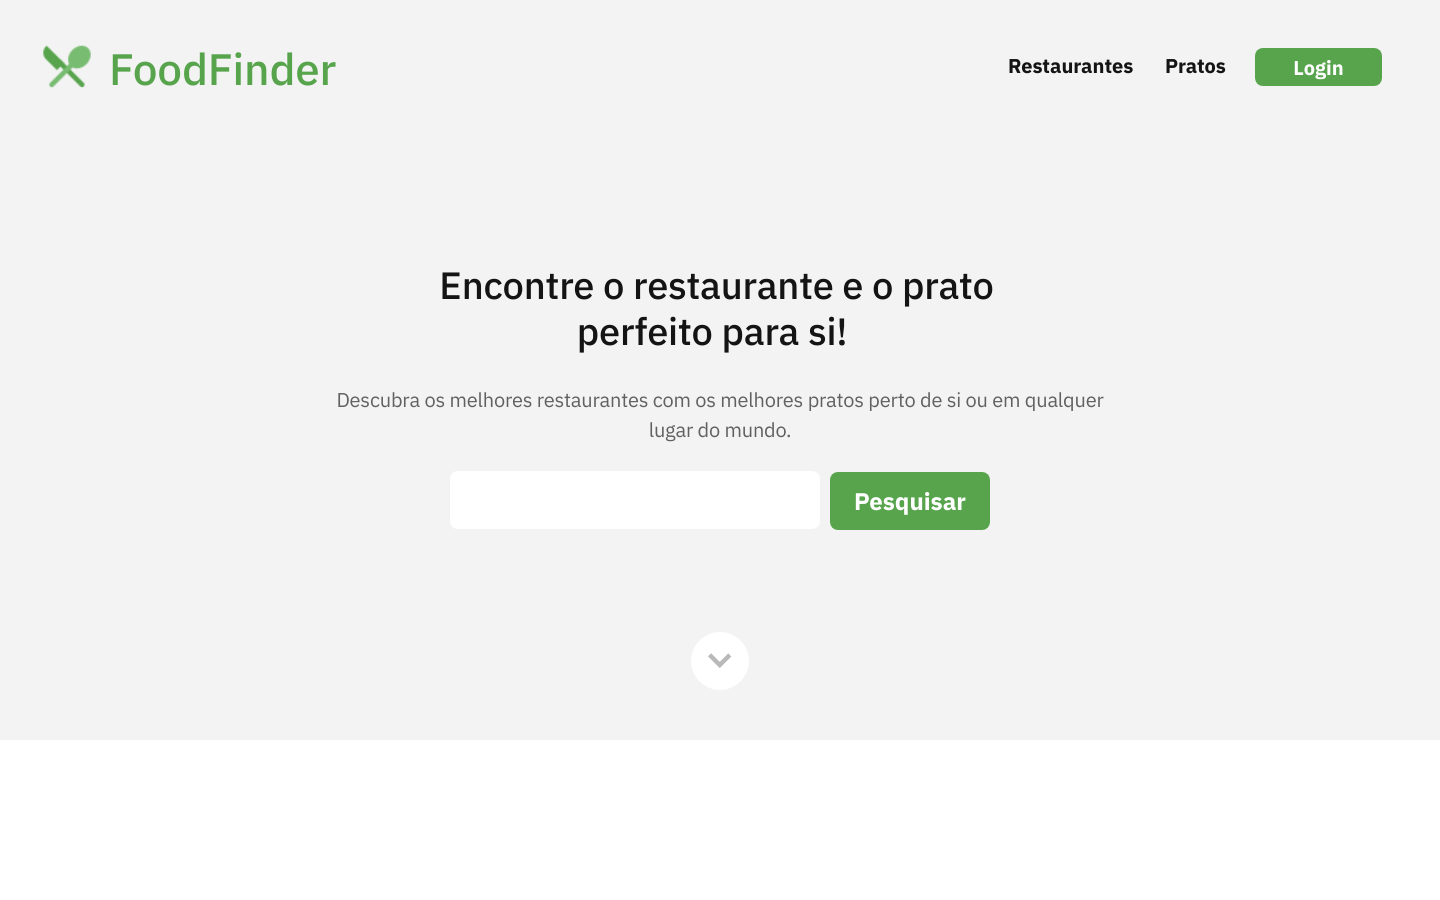
\includegraphics[scale=0.25]{1.1-Screen1}	
	\end{center}
	\caption{Parte Superior da \textit{Home Page}.}
	\end{figure} 
	
	\begin{figure}[H]
	\begin{center}
	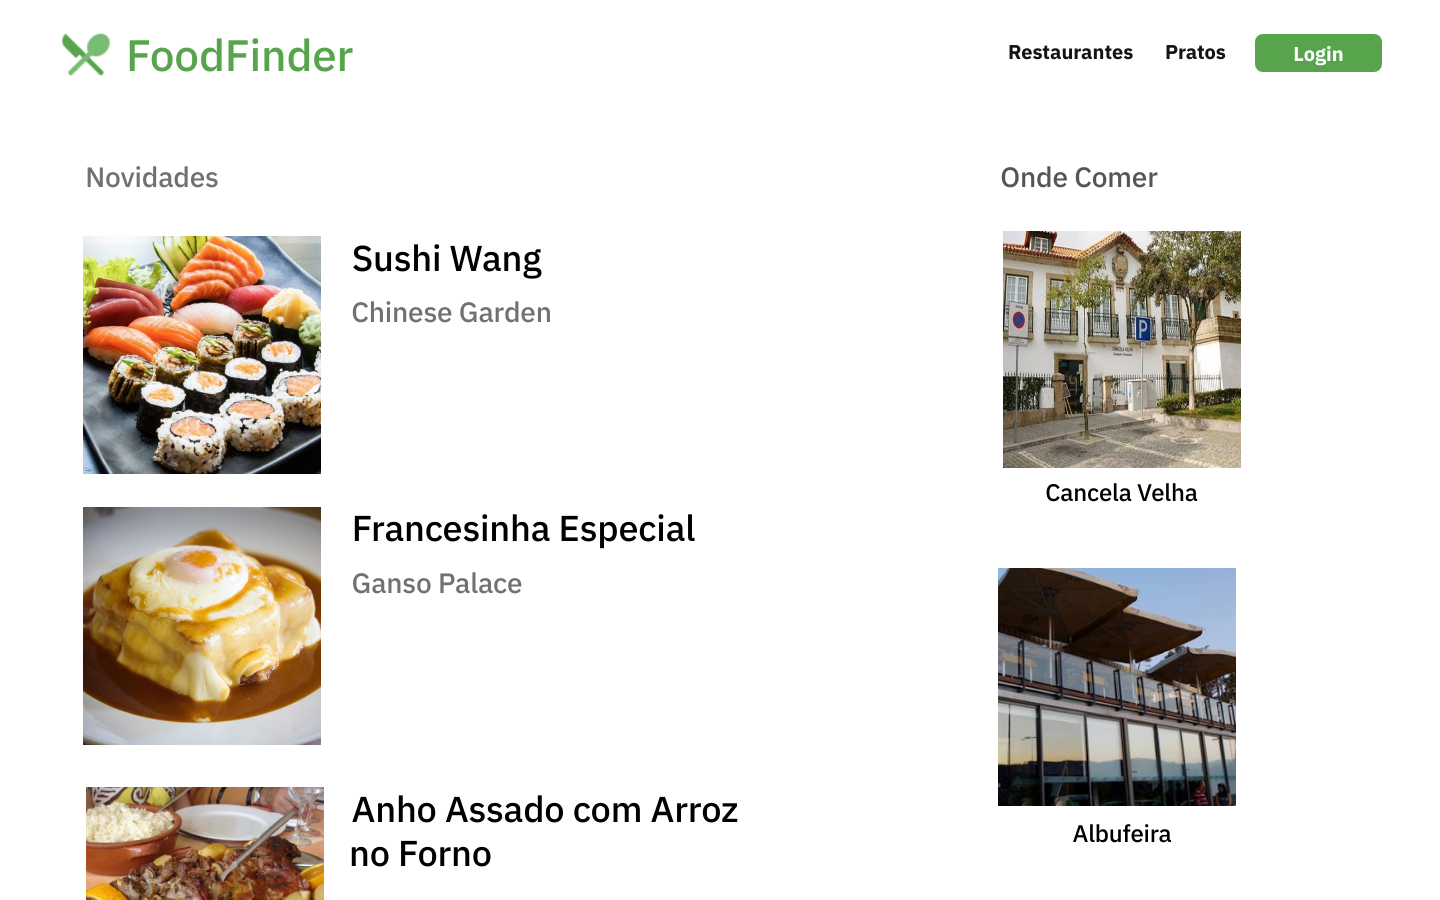
\includegraphics[scale=0.25]{2.1-Screen2}	
	\end{center}
	\caption{Parte Média da \textit{Home Page}.}
	\end{figure} 
	
	\begin{figure}[H]
	\begin{center}
	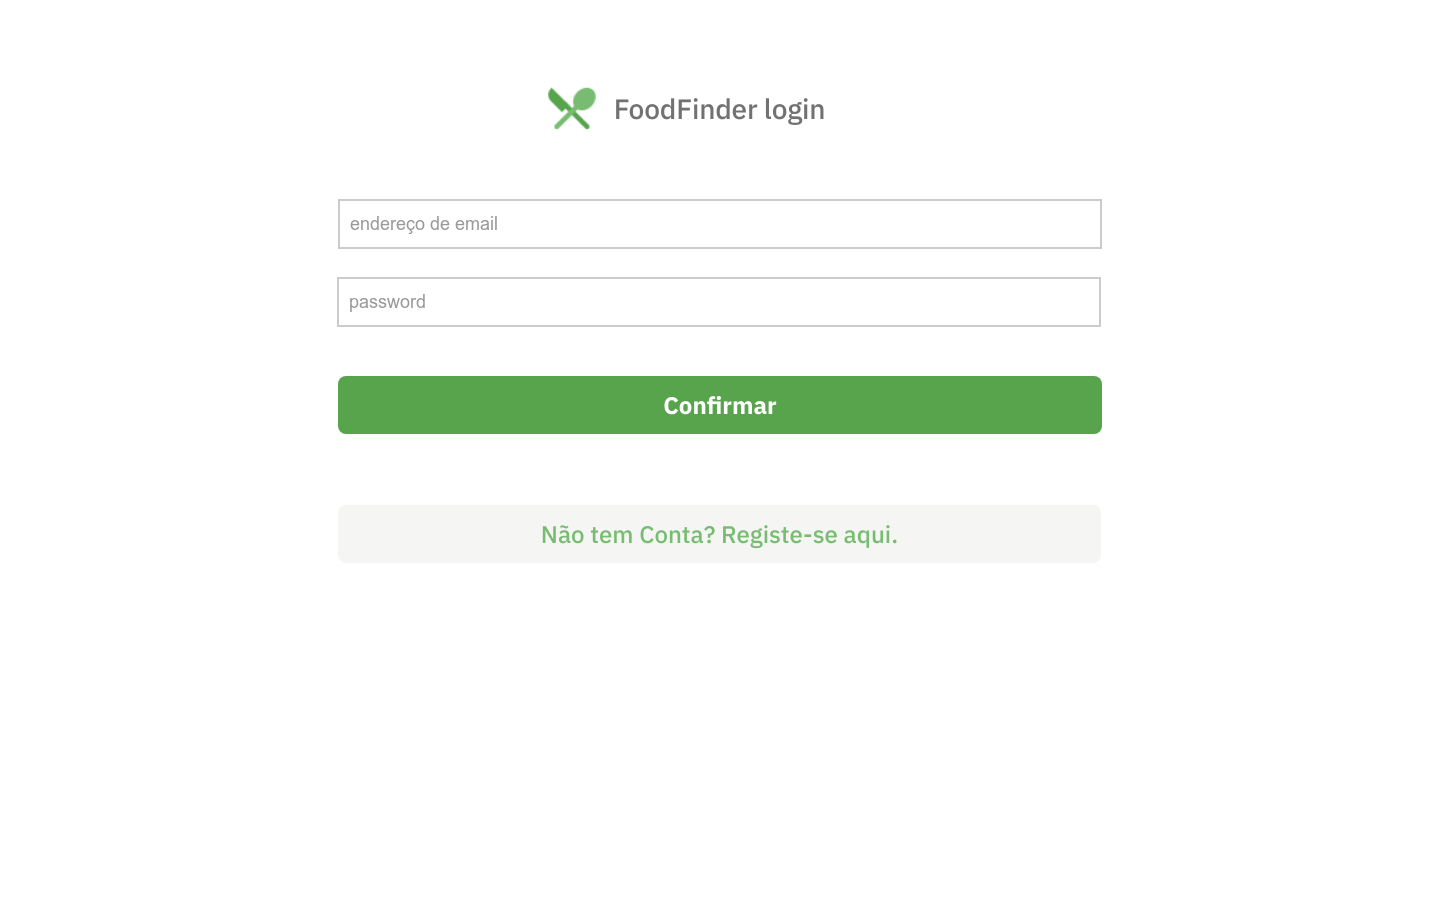
\includegraphics[scale=0.25]{3.1-Screen3}	
	\end{center}
	\caption{Interface para \textit{login}.}
	\end{figure} 
	
	\begin{figure}[H]
	\begin{center}
	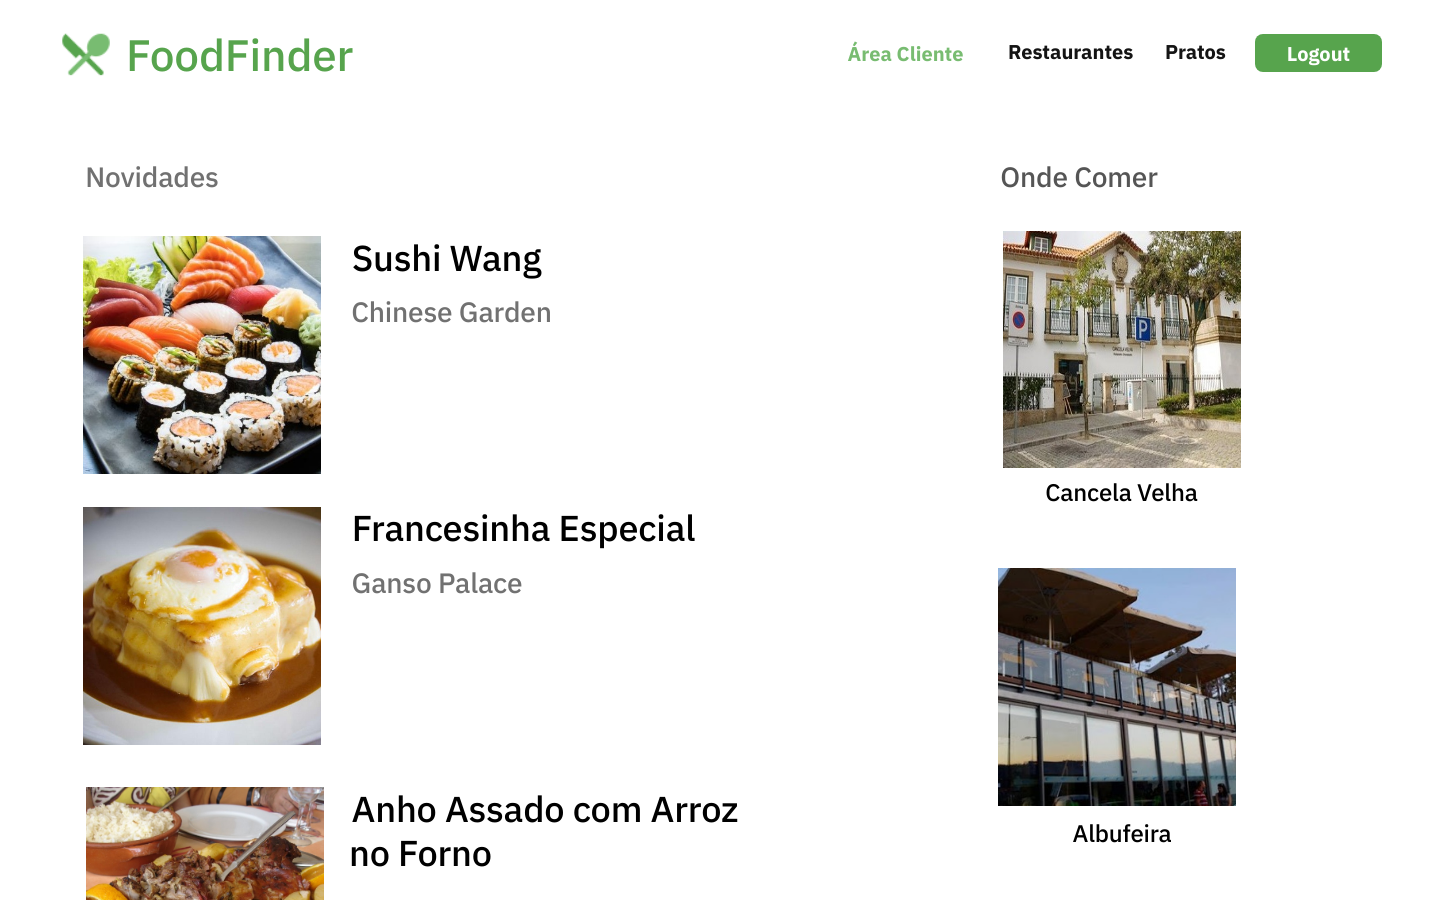
\includegraphics[scale=0.25]{7.1-Screen4}	
	\end{center}
	\caption{\textit{Homepage} após o \textit{login} de um utilizador.}
	\end{figure} 
	
	\begin{figure}[H]
	\begin{center}
	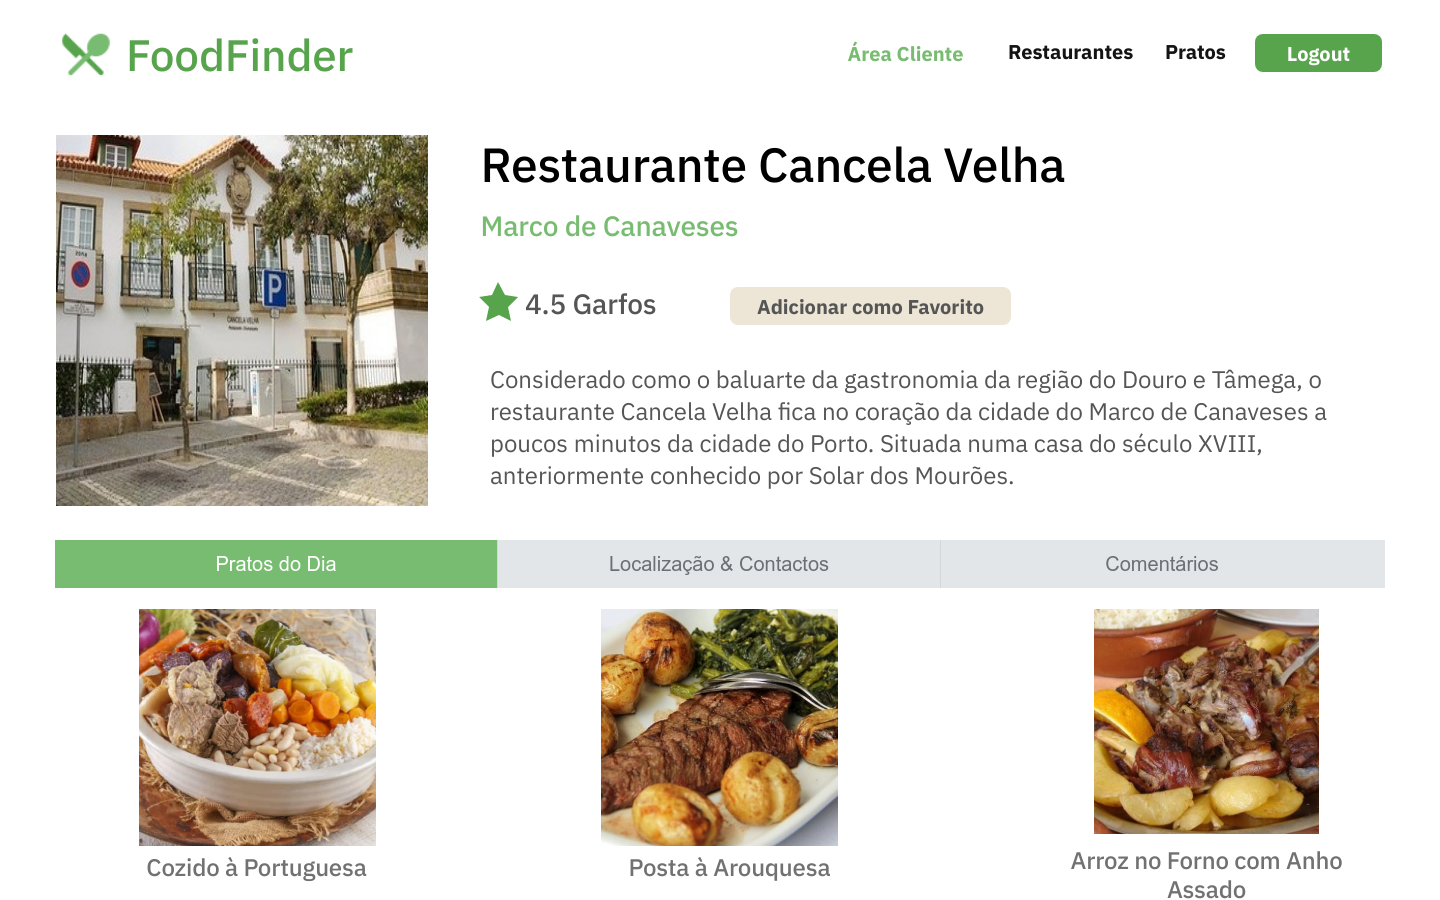
\includegraphics[scale=0.25]{8.1-Screen5}	
	\end{center}
	\caption{Interface onde é possível consultar informação do restaurante e os seus pratos do dia ativos.}
	\end{figure} 
	
	\begin{figure}[H]
	\begin{center}
	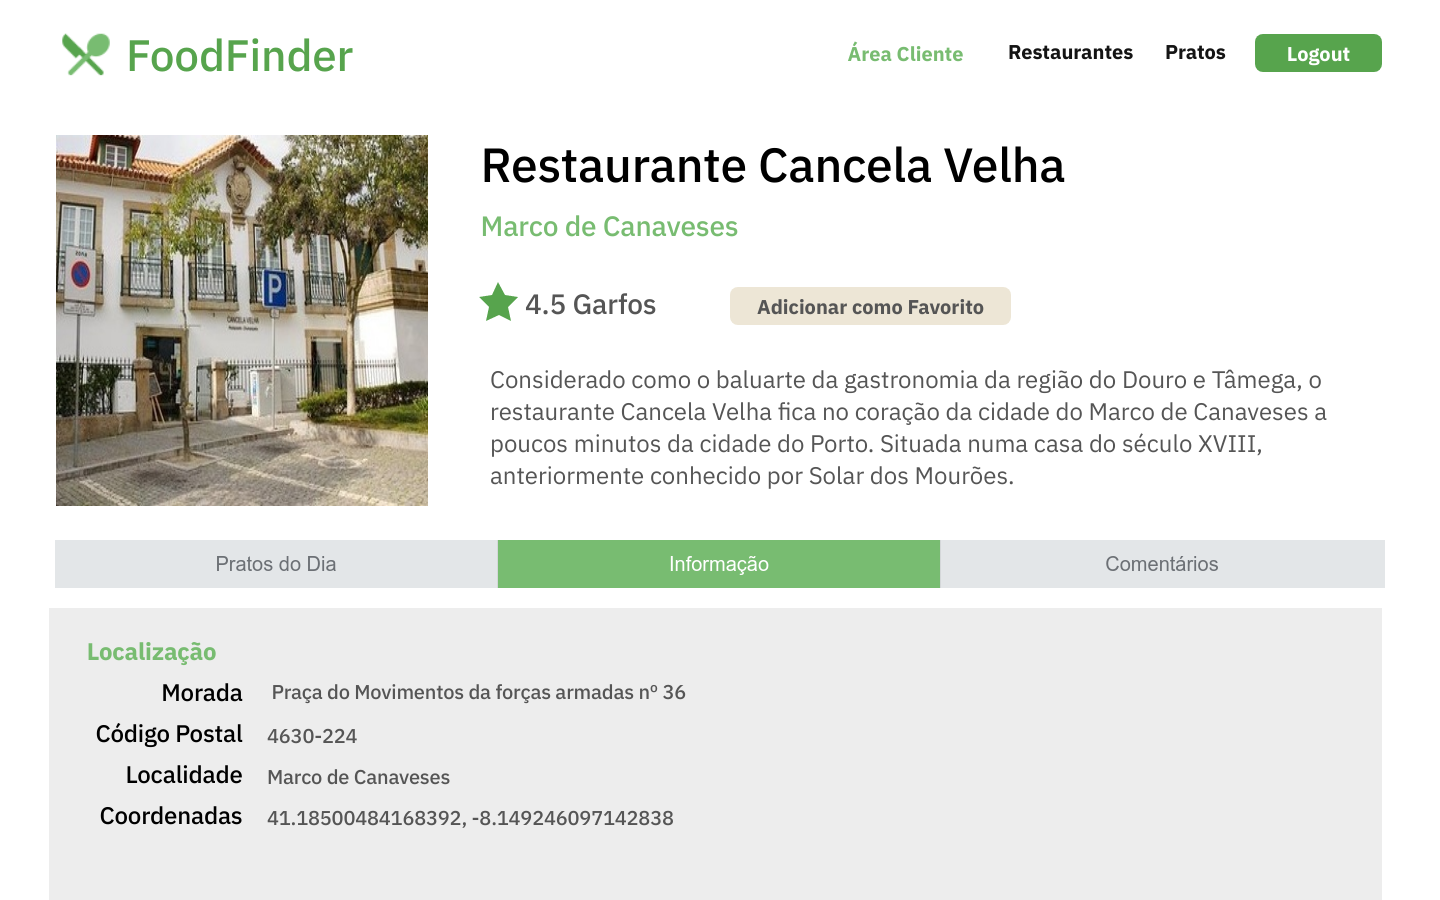
\includegraphics[scale=0.25]{9.1-Screen6}	
	\end{center}
	\caption{Interface onde é possível consultar informação do restaurante e a sua informação.}
	\end{figure} 
	
	\begin{figure}[H]
	\begin{center}
	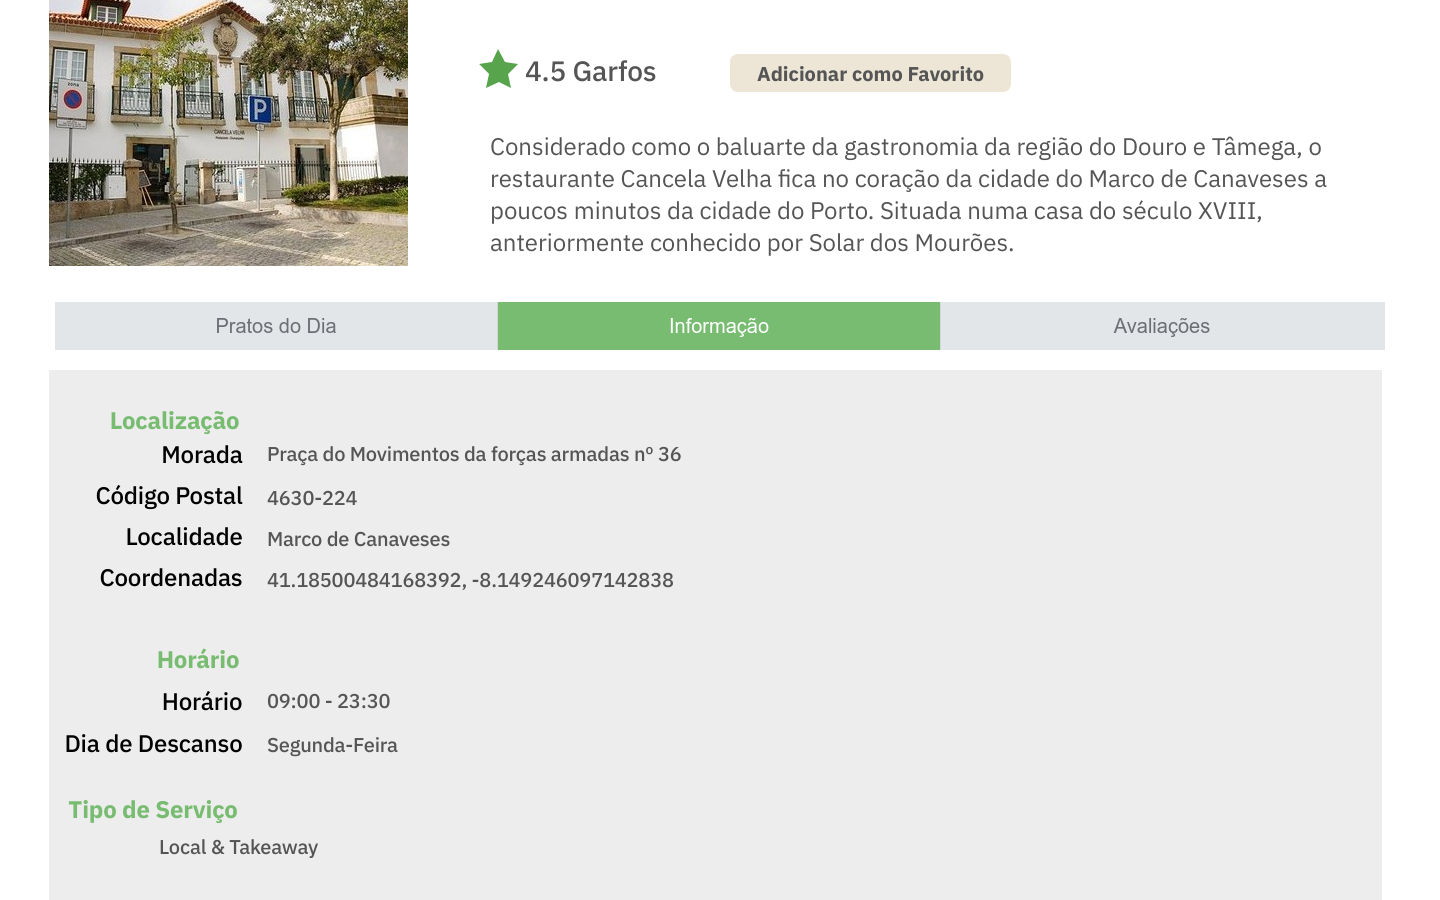
\includegraphics[scale=0.25]{10.1-Screen7}	
	\end{center}
	\caption{Interface onde é possível consultar informação do restaurante e os seus comentários restaurante. Note-se que se encontra em falta um botão para que o utilizador possa avaliar e comentar o restaurante.}
	\end{figure} 
	
	\begin{figure}[H]
	\begin{center}
	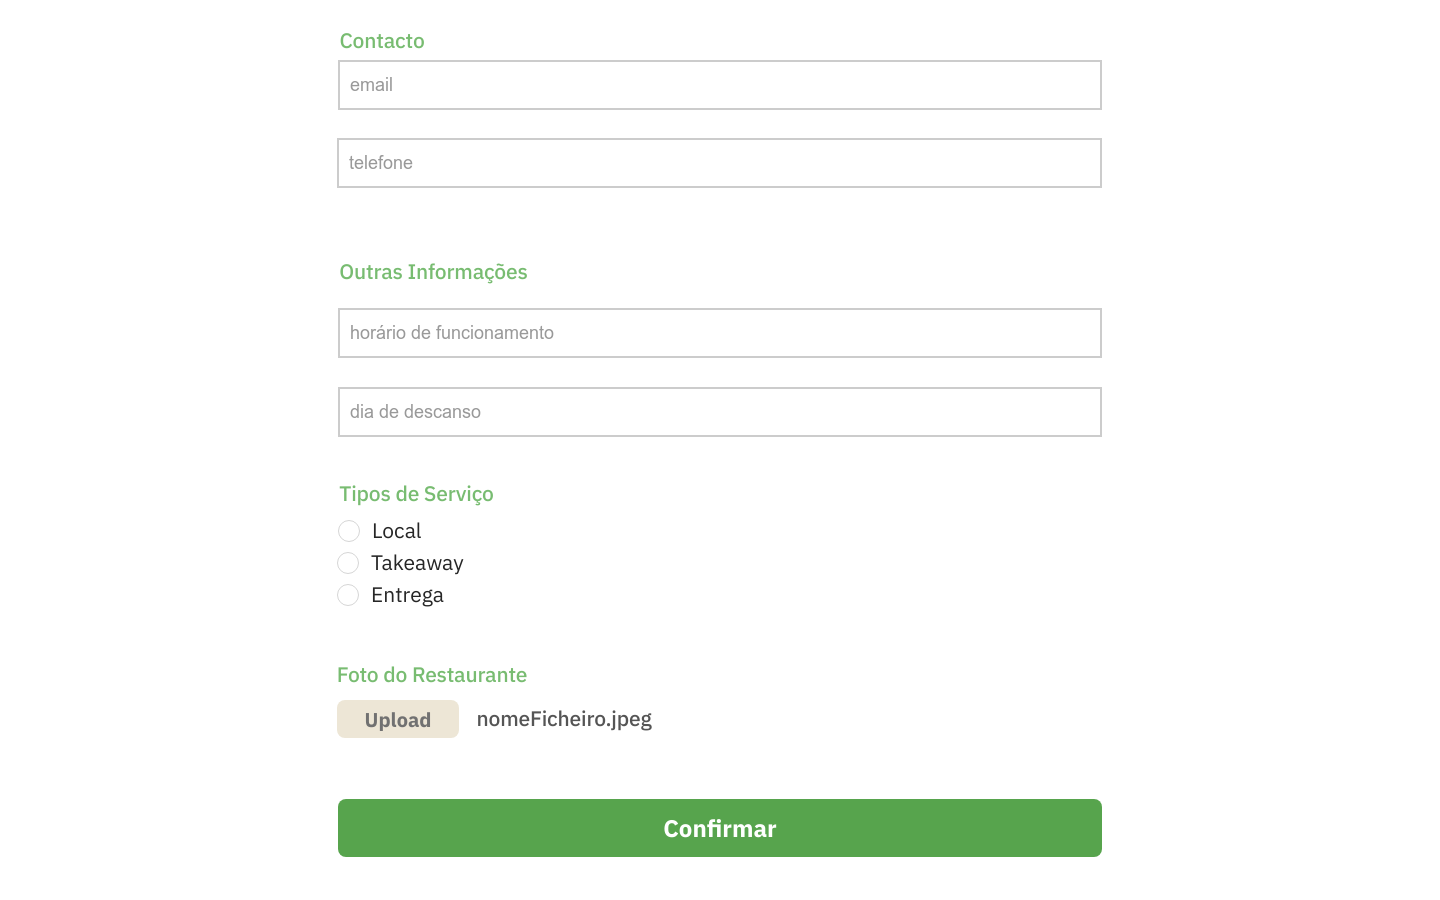
\includegraphics[scale=0.25]{6.1-Screen12}	
	\end{center}
	\caption{Interface que possibilita a pesquisa de restaurantes e pratos do dia.}
	\end{figure} 

	\begin{figure}[H]
	\begin{center}
	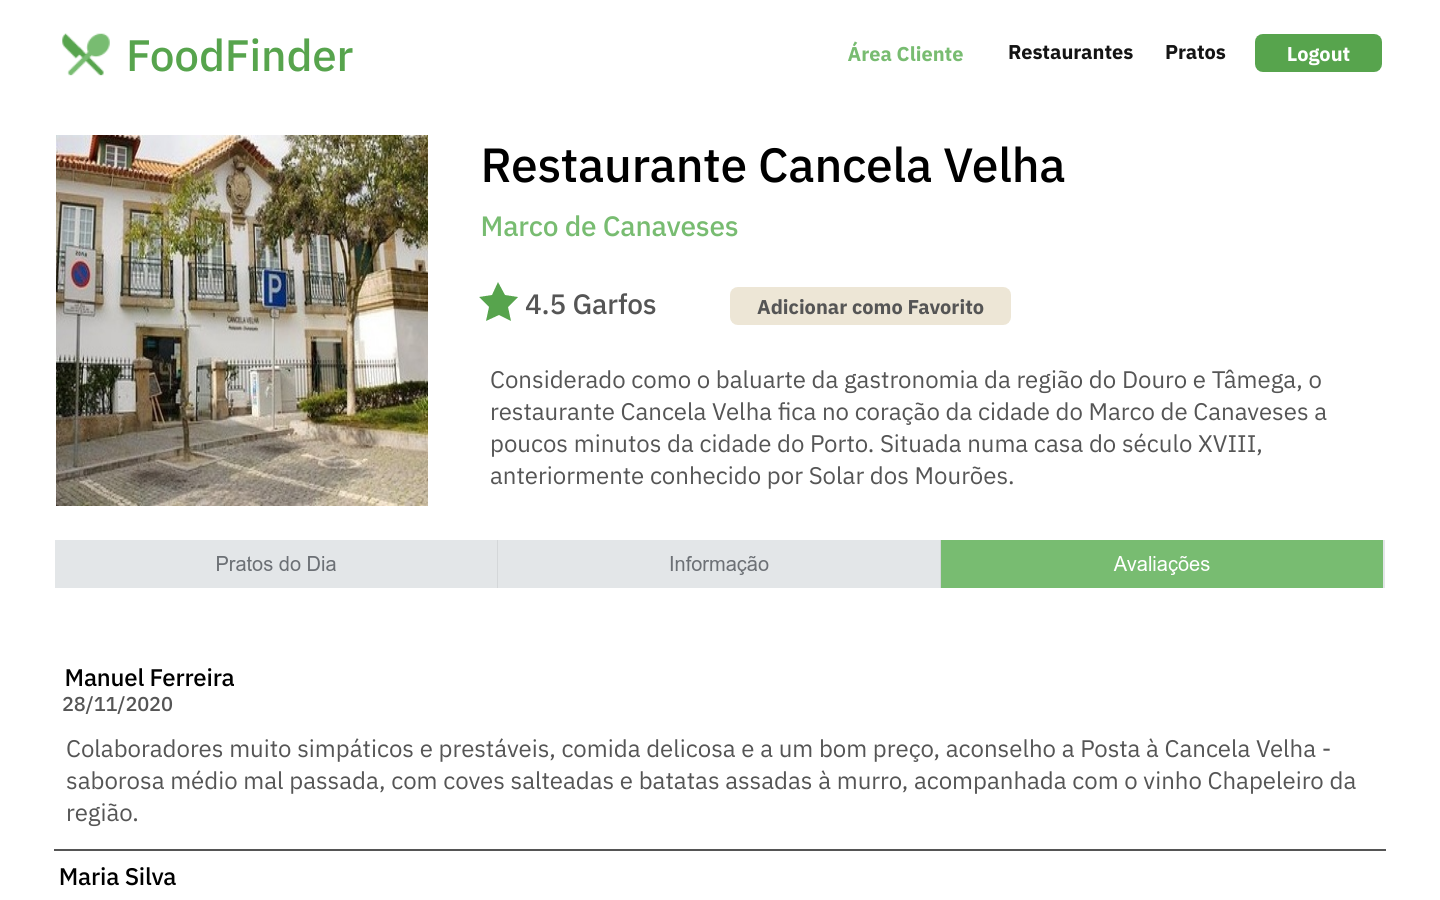
\includegraphics[scale=0.25]{11.1-Screen8}	
	\end{center}
	\caption{Interface que possibilita o registo de um utilizador.}
	\end{figure} 
	
	\begin{figure}[H]
	\begin{center}
	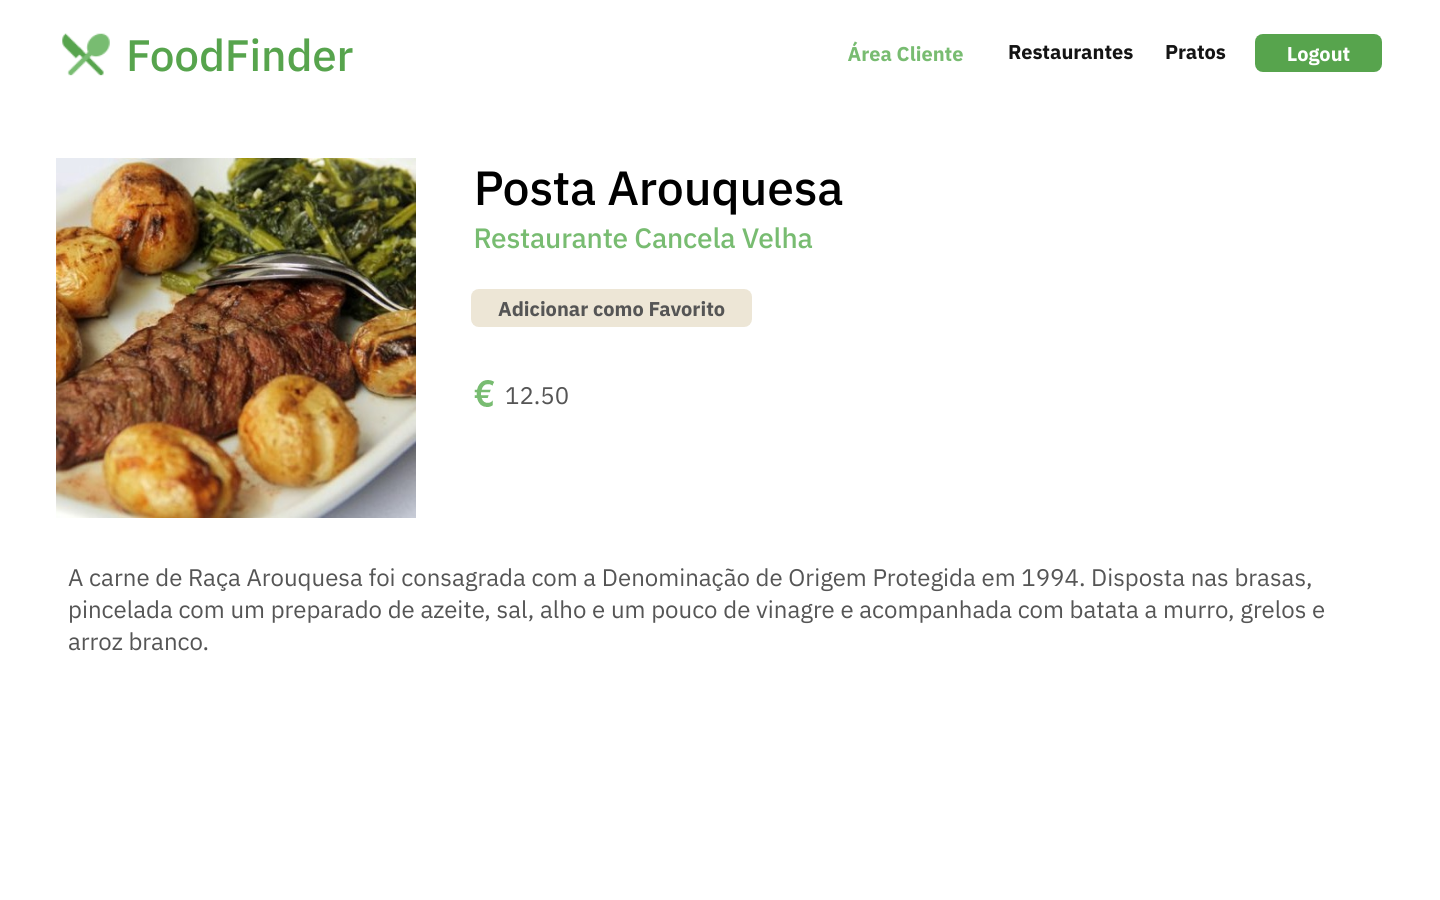
\includegraphics[scale=0.25]{12.1-Screen9}	
	\end{center}
	\caption{Interface que apresenta formulário seguinte para o registo de informações especificas de um restaurante.}
	\end{figure} 
	
	\begin{figure}[H]
	\begin{center}
	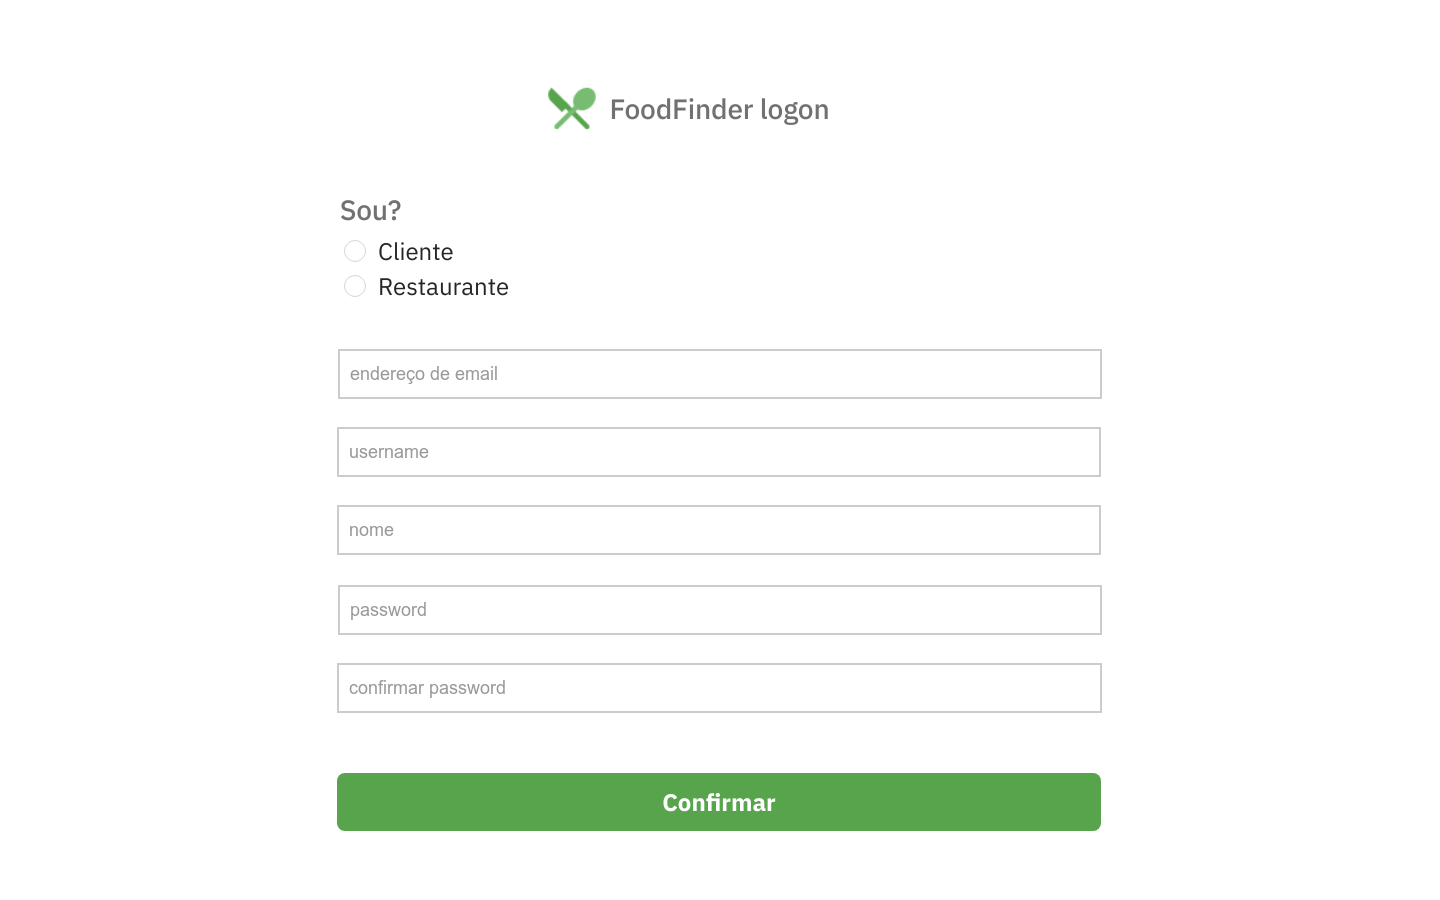
\includegraphics[scale=0.25]{4.1-Screen10}	
	\end{center}
	\caption{Continuação da interface que apresenta formulário seguinte para o registo de informações especificas de um restaurante.}
	\end{figure} 
	
	\begin{figure}[H]
	\begin{center}
	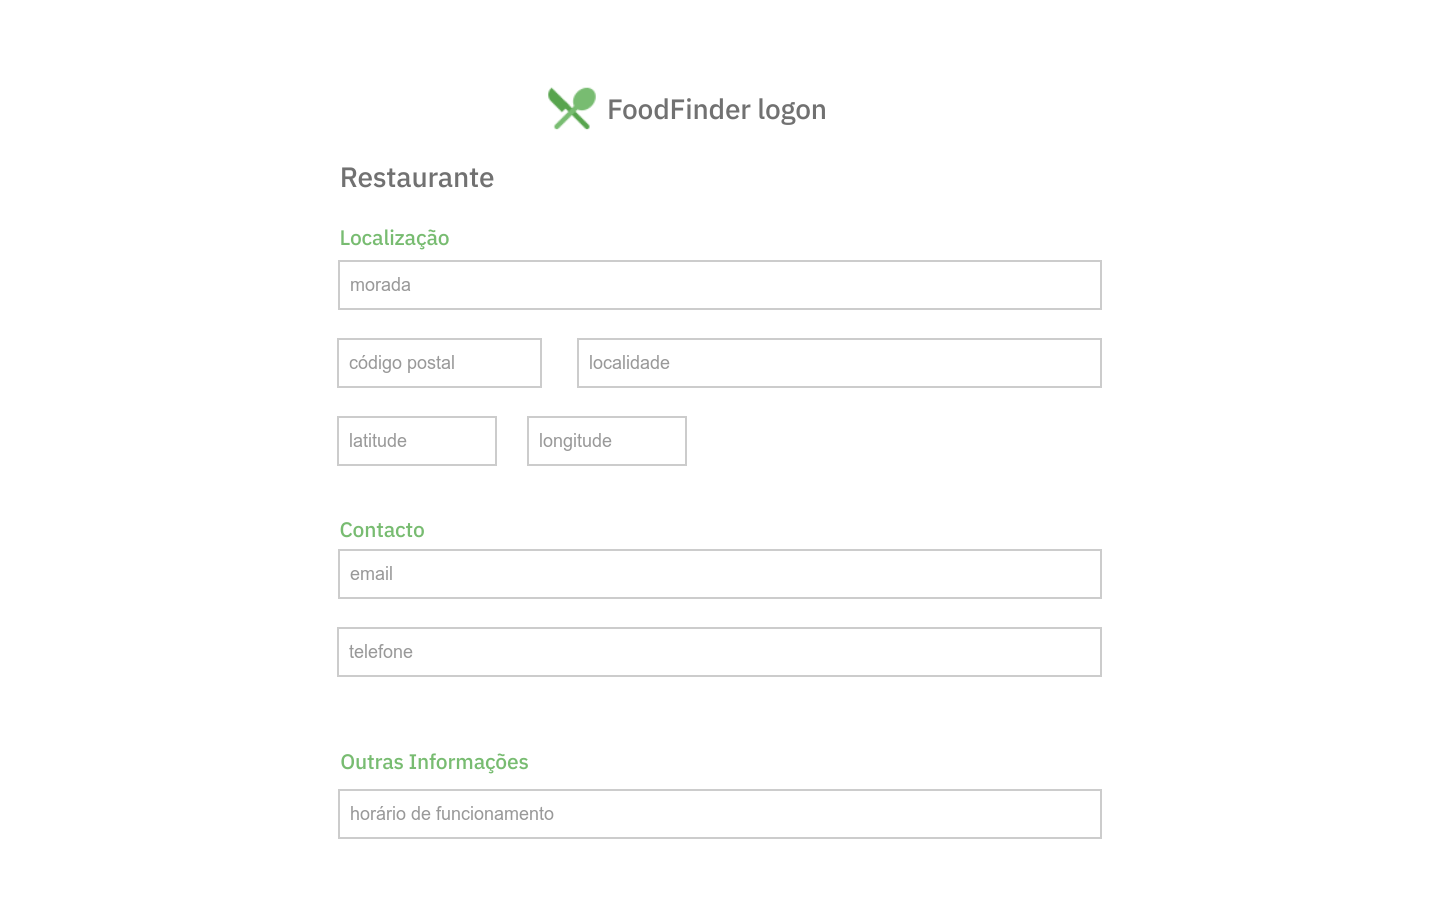
\includegraphics[scale=0.25]{5.1-Screen11}	
	\end{center}
	\caption{Interface apresenta o menu da Área Cliente.}
	\end{figure} 

	
	\begin{figure}[H]
	\begin{center}
	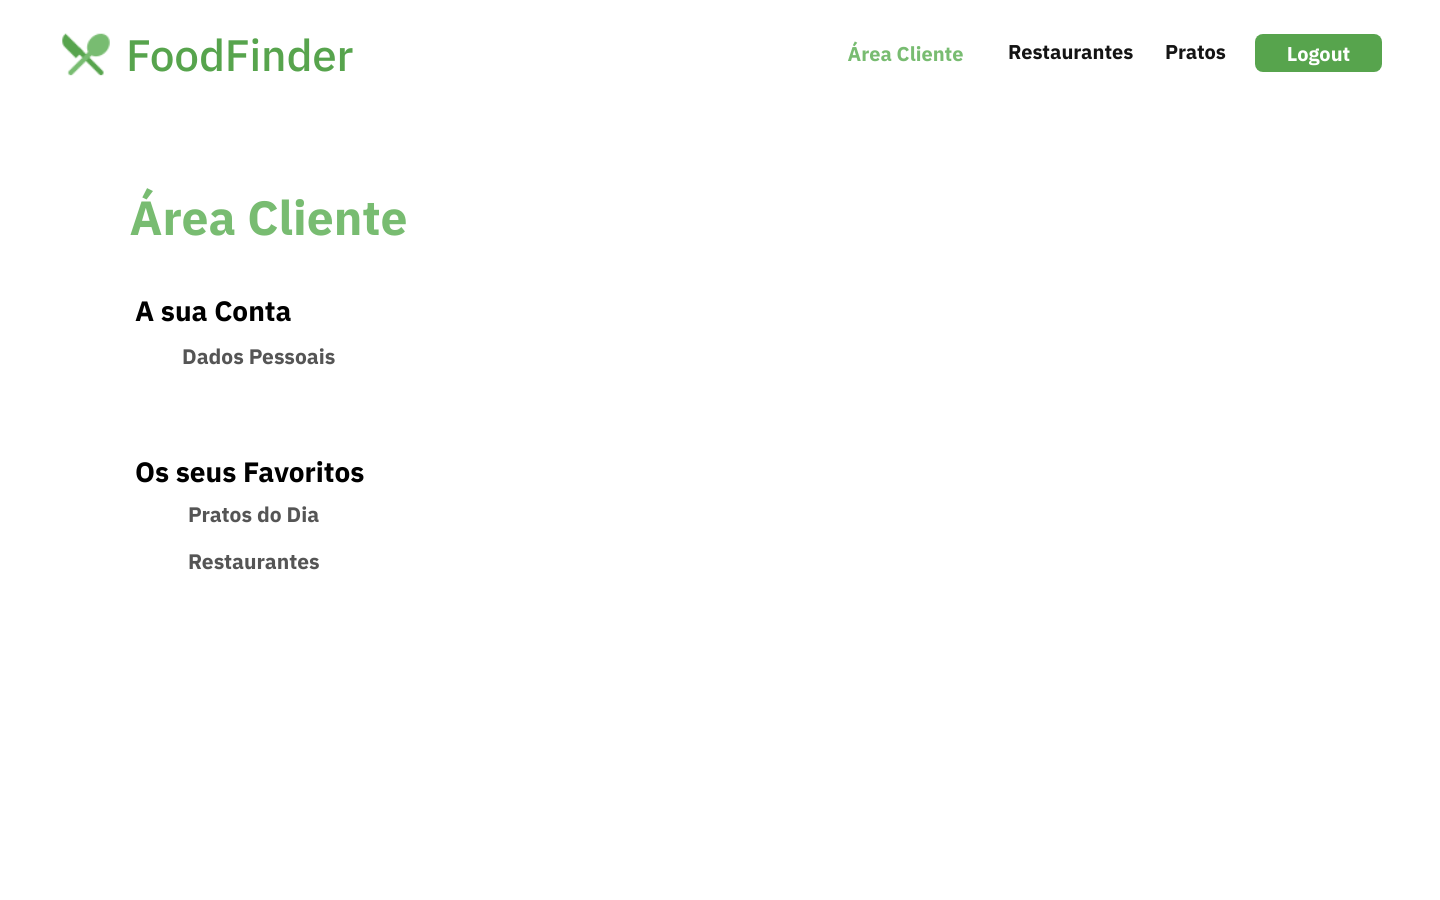
\includegraphics[scale=0.25]{6.1-Screen13}	
	\end{center}
	\caption{Interface que apresenta informações de um restaurante.}
	\end{figure} 
	
	\begin{figure}[H]
	\begin{center}
	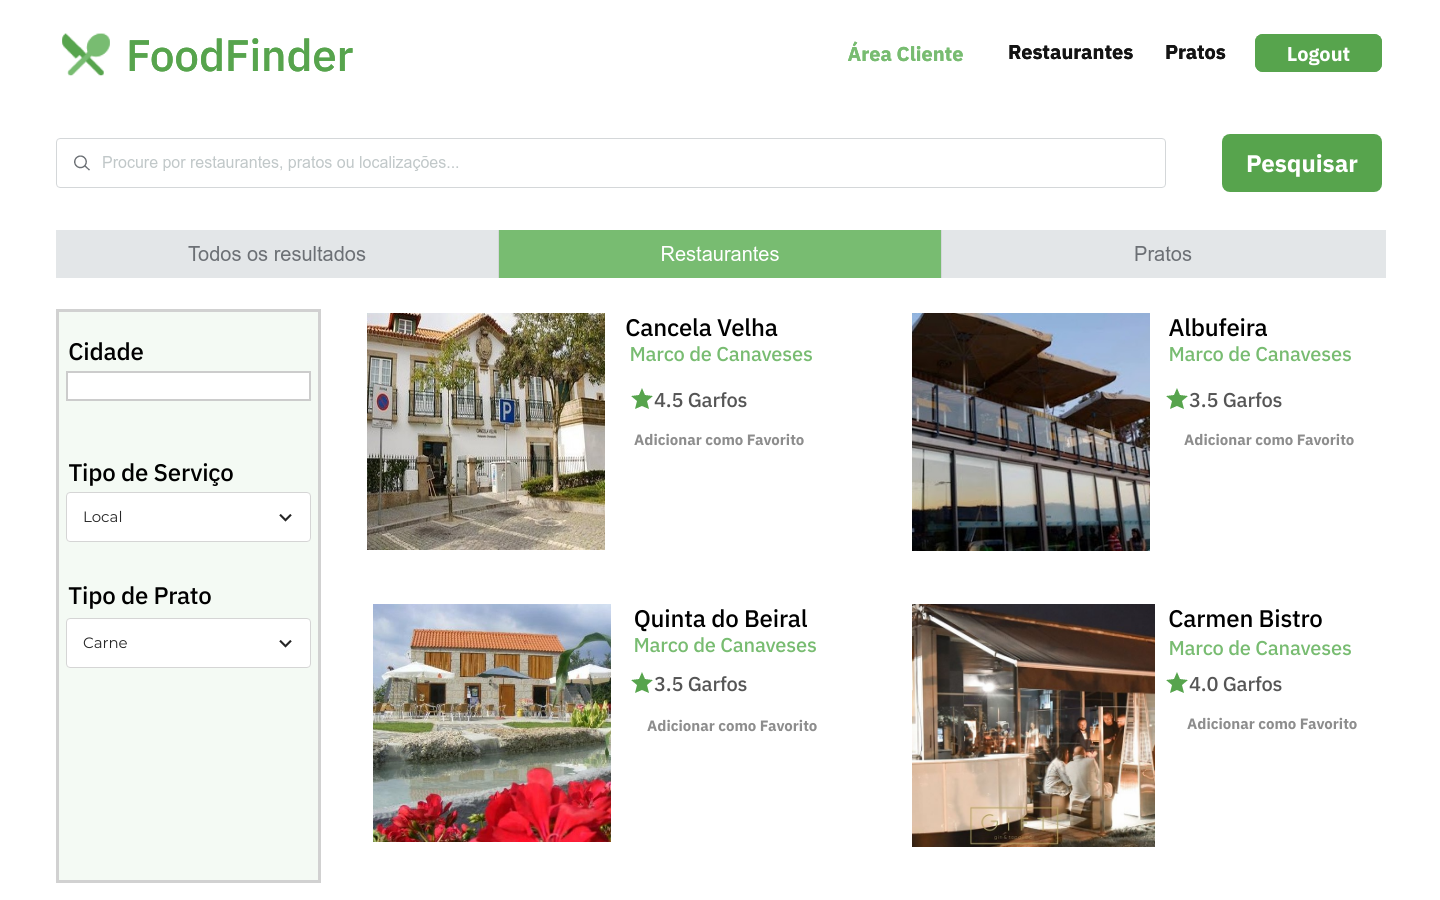
\includegraphics[scale=0.25]{14.1-Screen14}	
	\end{center}
	\caption{Interface que apresenta informações de um prato.}
	\end{figure}
	
	\begin{figure}[H]
	\begin{center}
	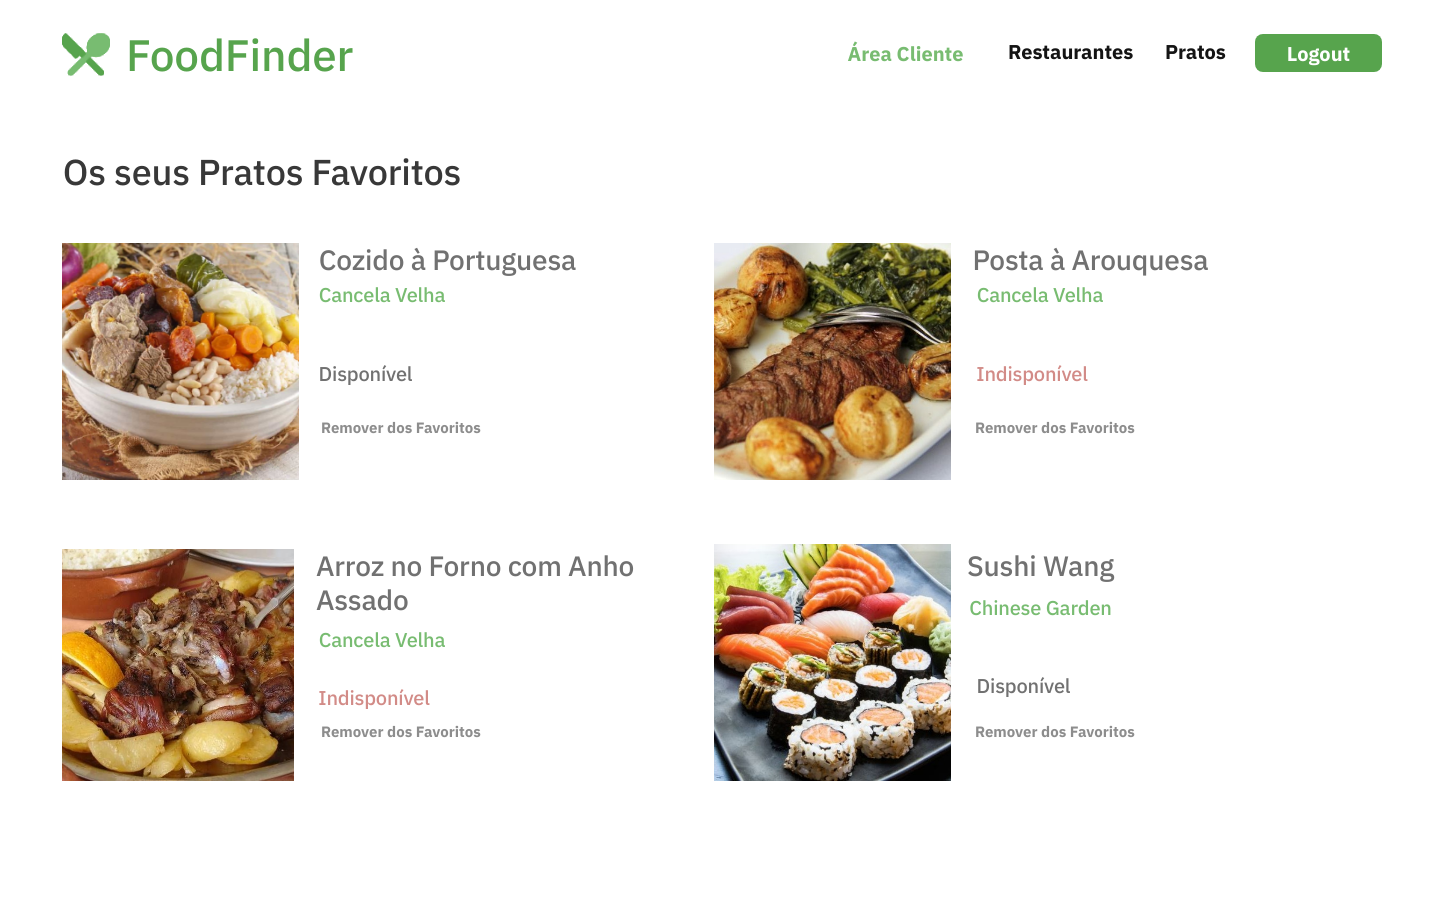
\includegraphics[scale=0.25]{15.1-Screen15}	
	\end{center}
	\caption{Interface que apresenta informações de um restaurante.}
	\end{figure} 
	
	\begin{figure}[H]
	\begin{center}
	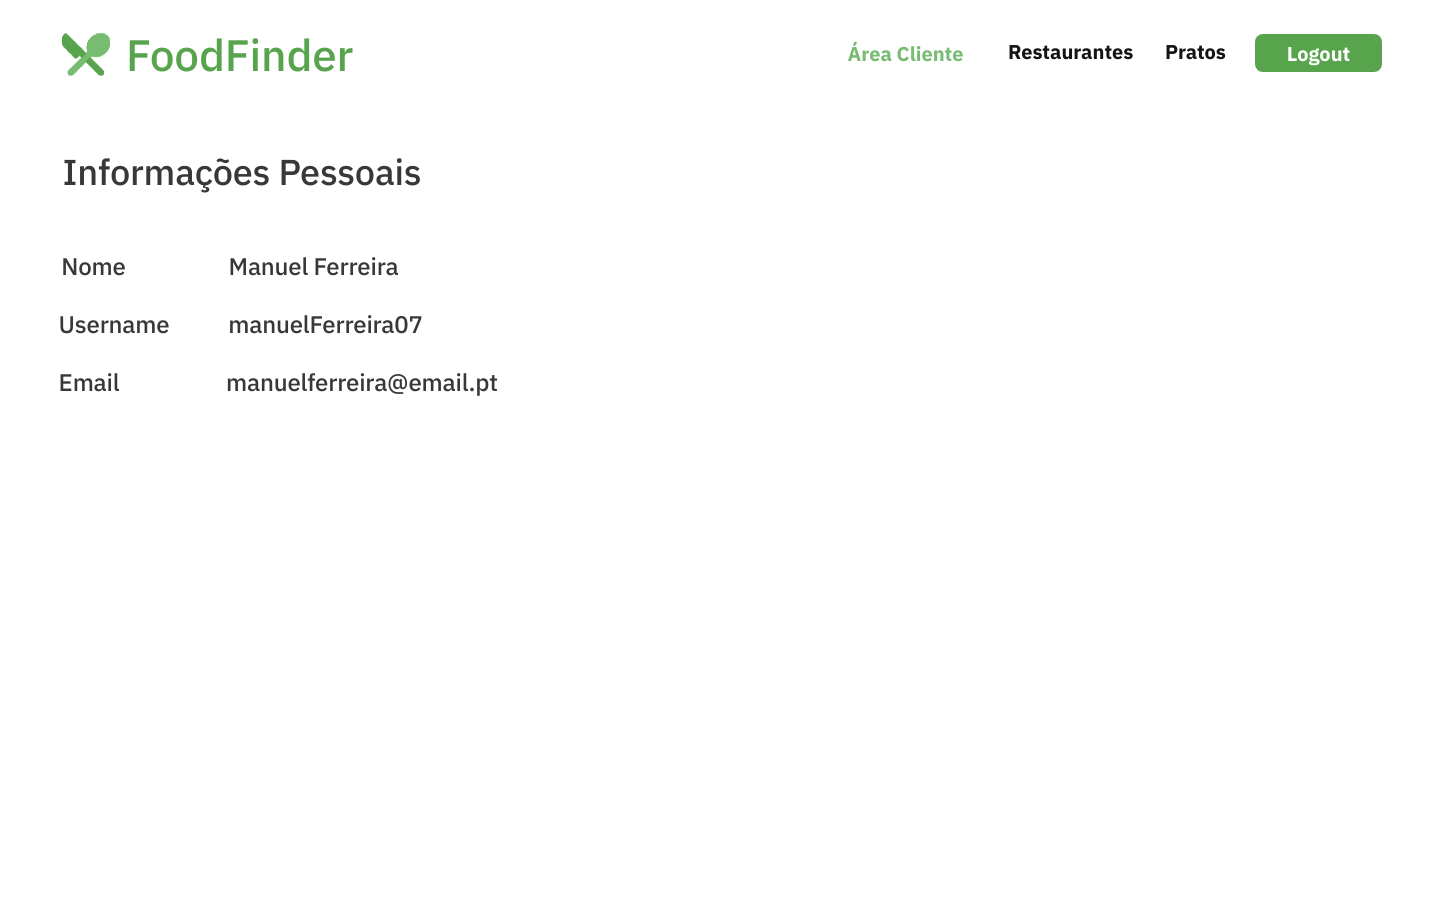
\includegraphics[scale=0.25]{16.1-Screen16}	
	\end{center}
	\caption{Interface que possibilita a um utilizador consultar a sua própria informação.}
	\end{figure}  

	
	
	
	
	
	
\section{Interfaces Específicas do Restaurante}	

	\begin{figure}[H]
	\begin{center}
	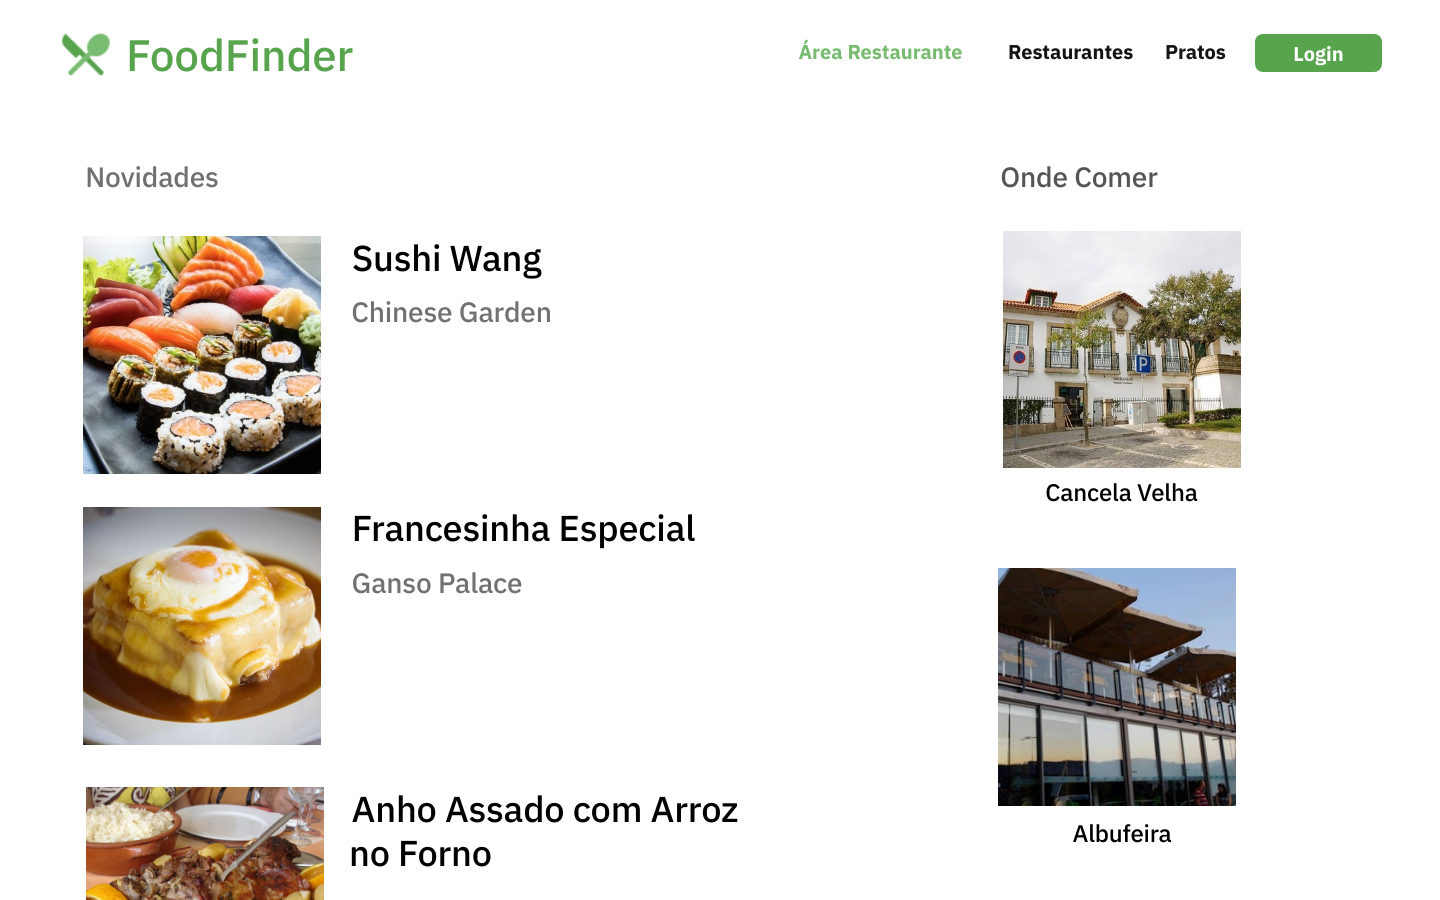
\includegraphics[scale=0.25]{1.1-Menu_principal_restaurante}	
	\end{center}
	\caption{Interface que representa a homepage quando o utilizador fez login como restaurante.}
	\end{figure} 

	\begin{figure}[H]
	\begin{center}
	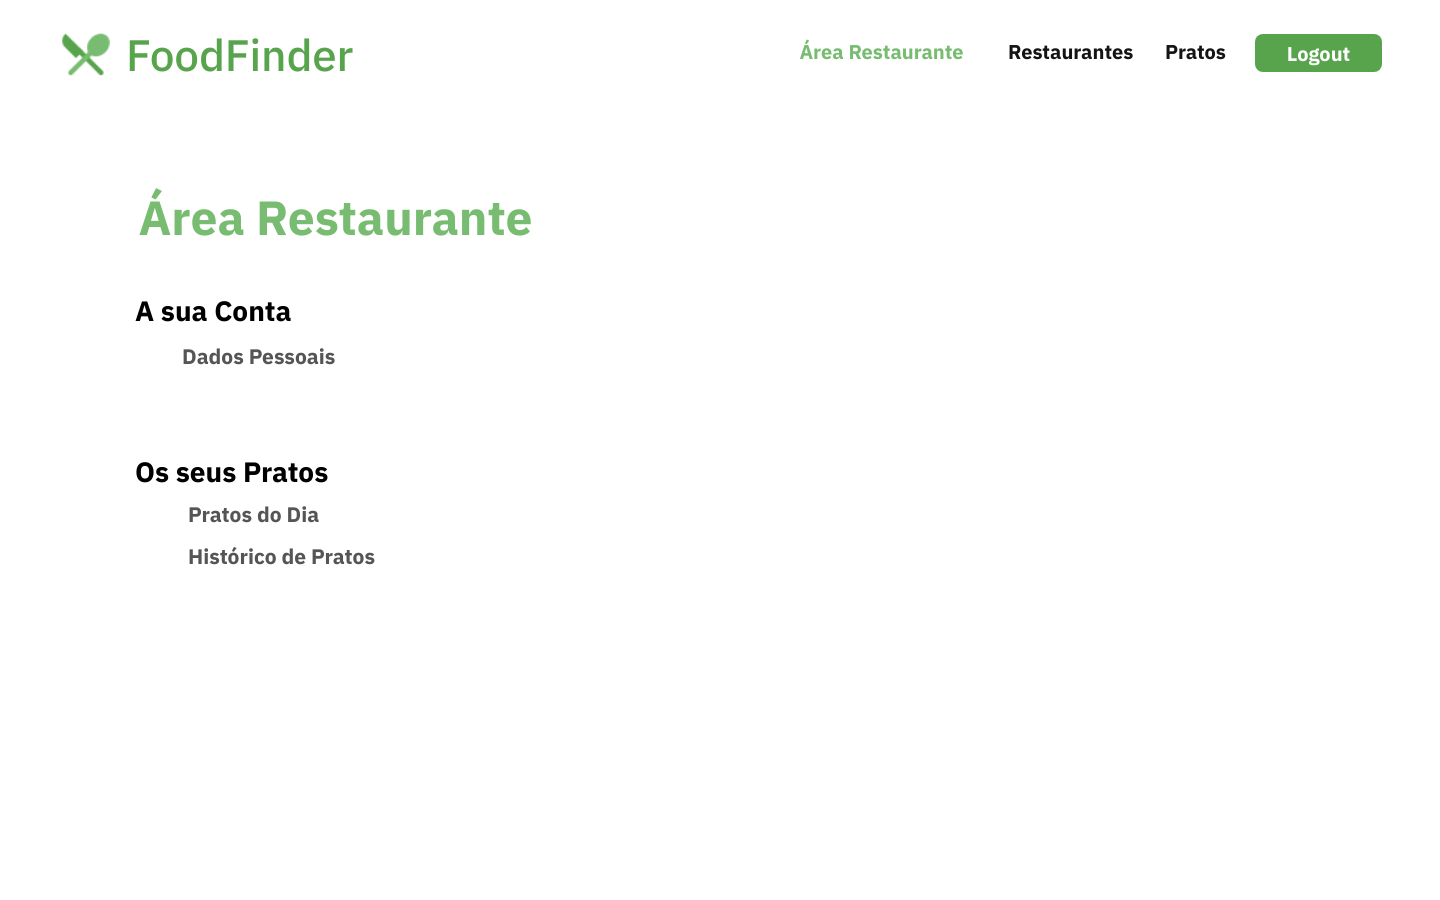
\includegraphics[scale=0.25]{2.1-Area_restaurante}	
	\end{center}
	\caption{Interface que apresenta o menu da Área Restaurante.}
	\end{figure} 
	
	\begin{figure}[H]
	\begin{center}
	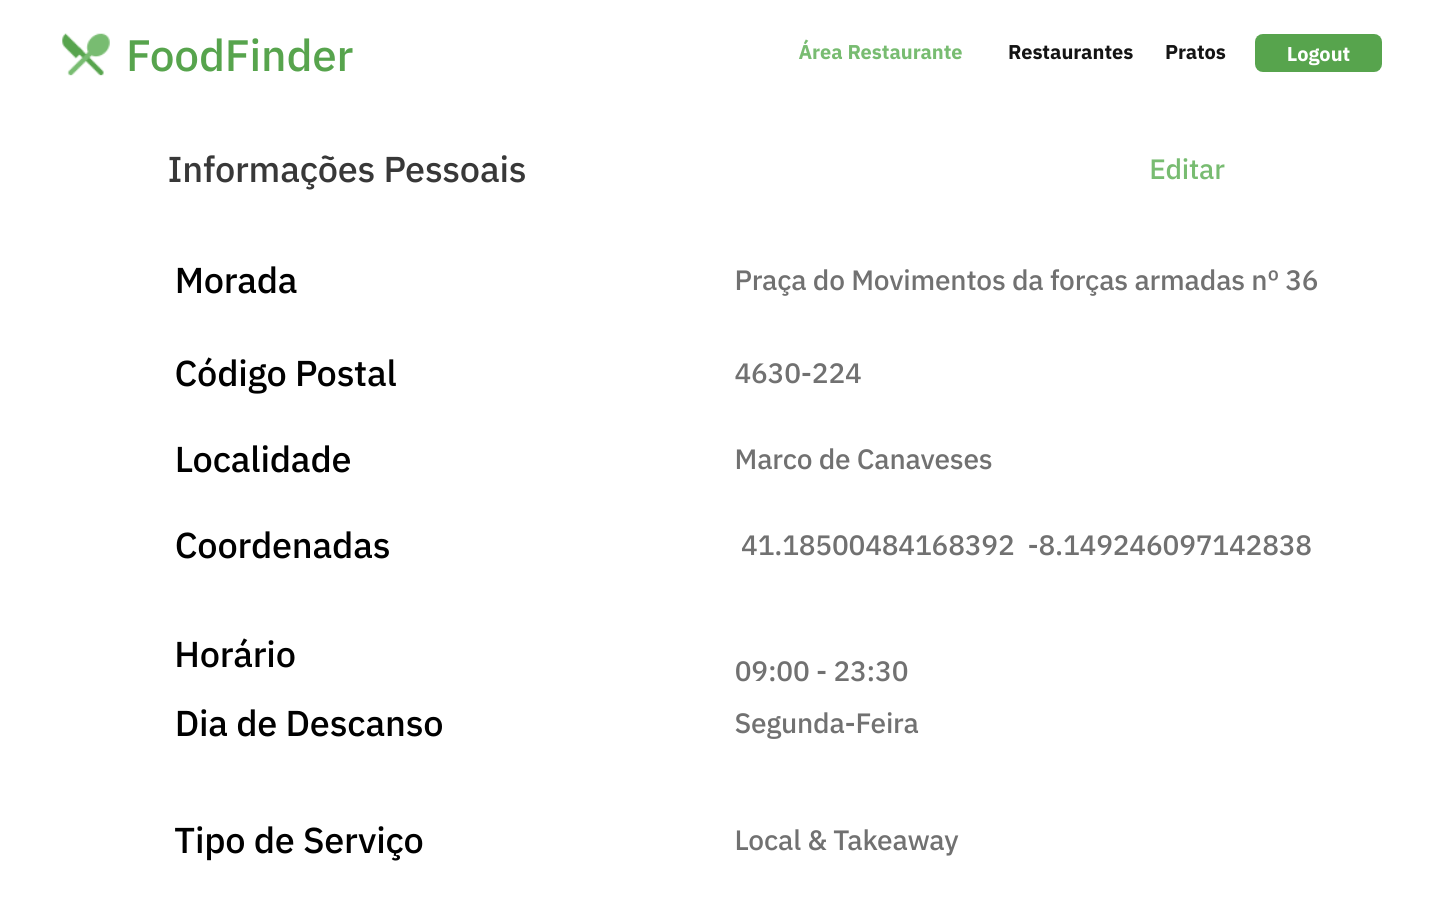
\includegraphics[scale=0.25]{3.1-Dados_Pessoais_restaurante}	
	\end{center}
	\caption{Interface que permite a um restaurante consultar a sua própria informação.}
	\end{figure} 
	
	\begin{figure}[H]
	\begin{center}
	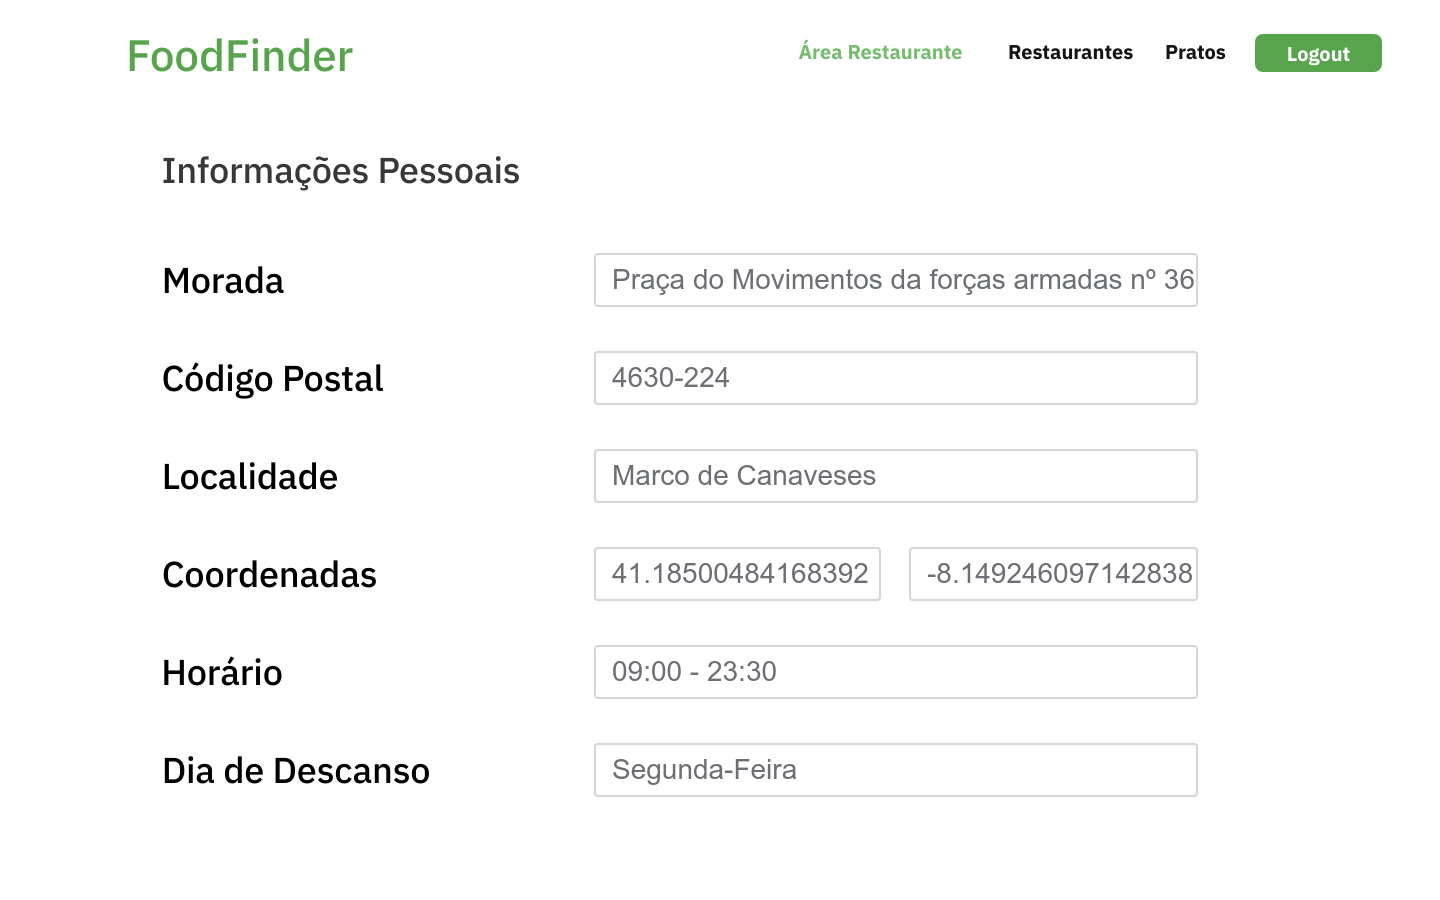
\includegraphics[scale=0.25]{4.1-Editar_Dados_restaurante_1}	
	\end{center}
	\caption{Interface que permite a um restaurante editar a sua própria informação.}
	\end{figure} 
	
	\begin{figure}[H]
	\begin{center}
	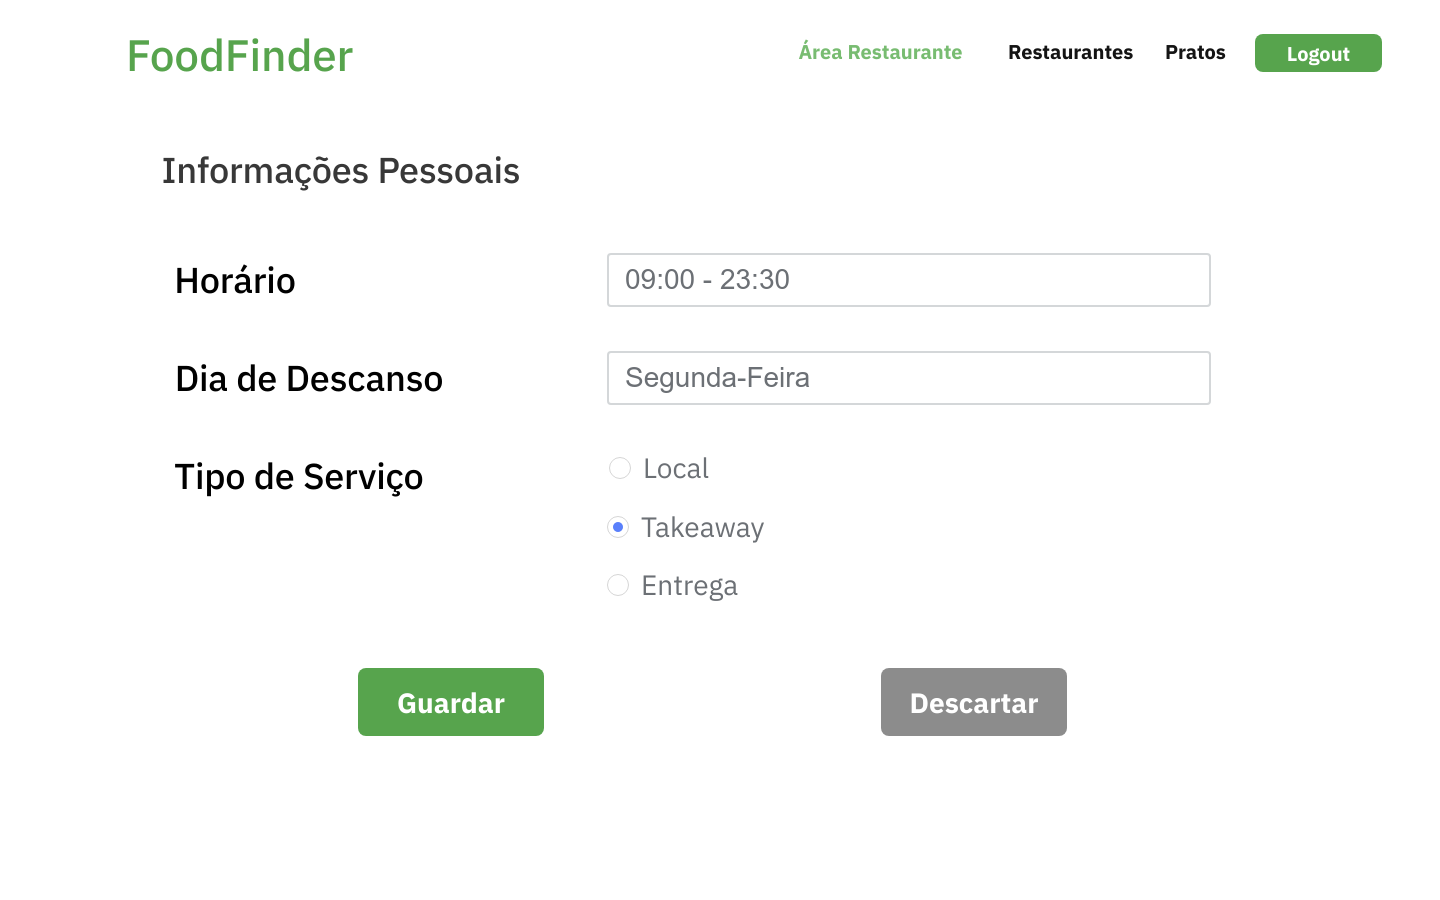
\includegraphics[scale=0.25]{5.1-Edtiar_Dados_restaurante_2}	
	\end{center}
	\caption{Continuação da interface que permite a um restaurante consultar a sua própria informação.}
	\end{figure} 

	\begin{figure}[H]
	\begin{center}
	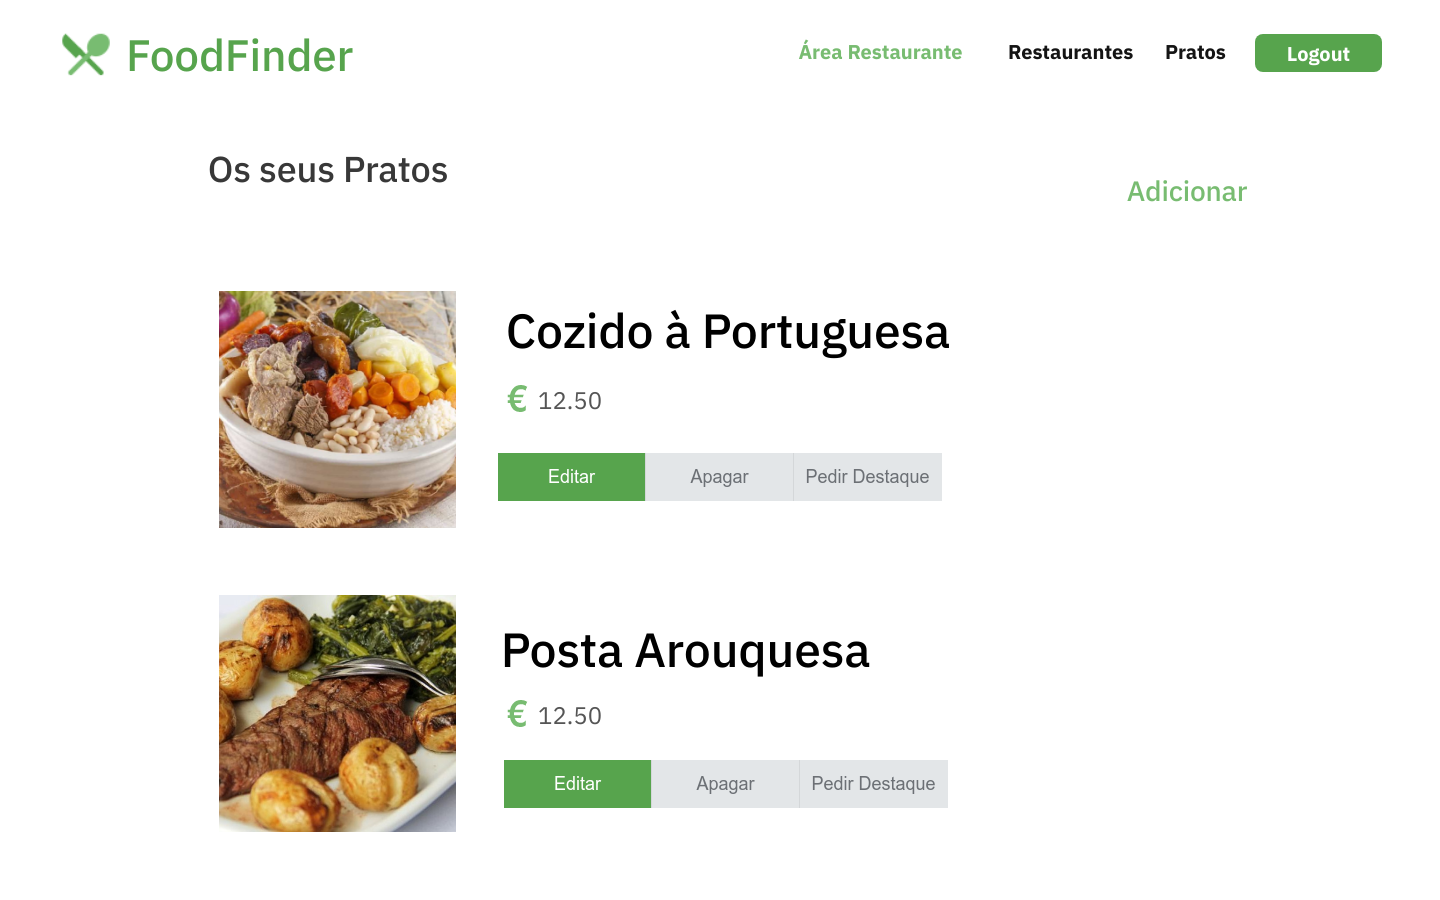
\includegraphics[scale=0.25]{6.1-Pratos_Dia_Ativos_restaurante_1}	
	\end{center}
	\caption{Interface que permite a um restaurante consultar os seus pratos ativos.}
	\end{figure}


	\begin{figure}[H]
	\begin{center}
	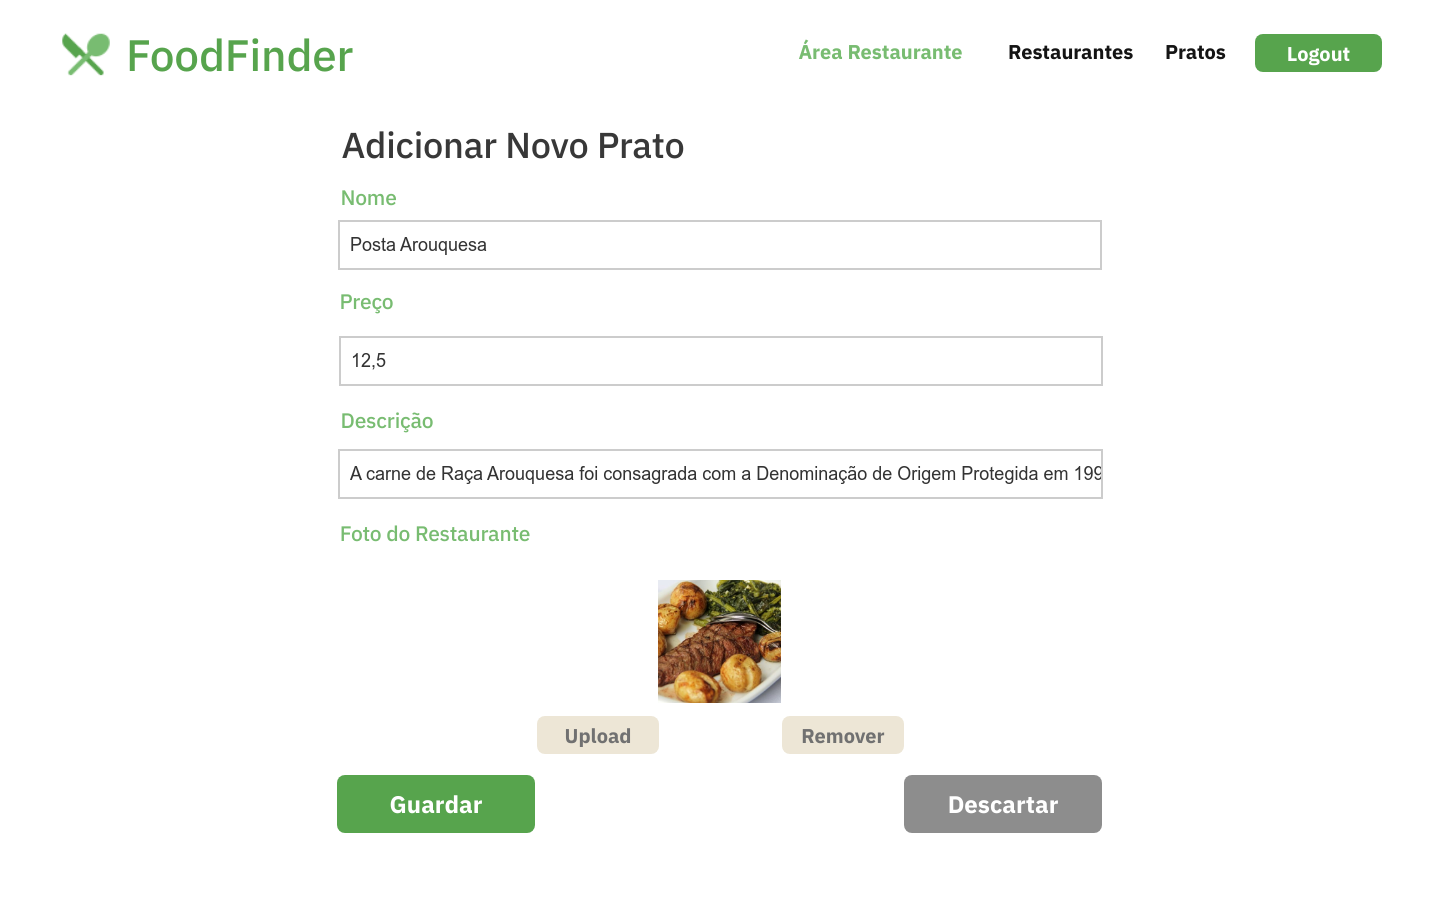
\includegraphics[scale=0.25]{9.1-Pratos_Dia_Ativos_Editar_restaurante}	
	\end{center}
	\caption{Interface que permite a um restaurante consultar os seus pratos anteriores.}
	\end{figure}
	
	\begin{figure}[H]
	\begin{center}
	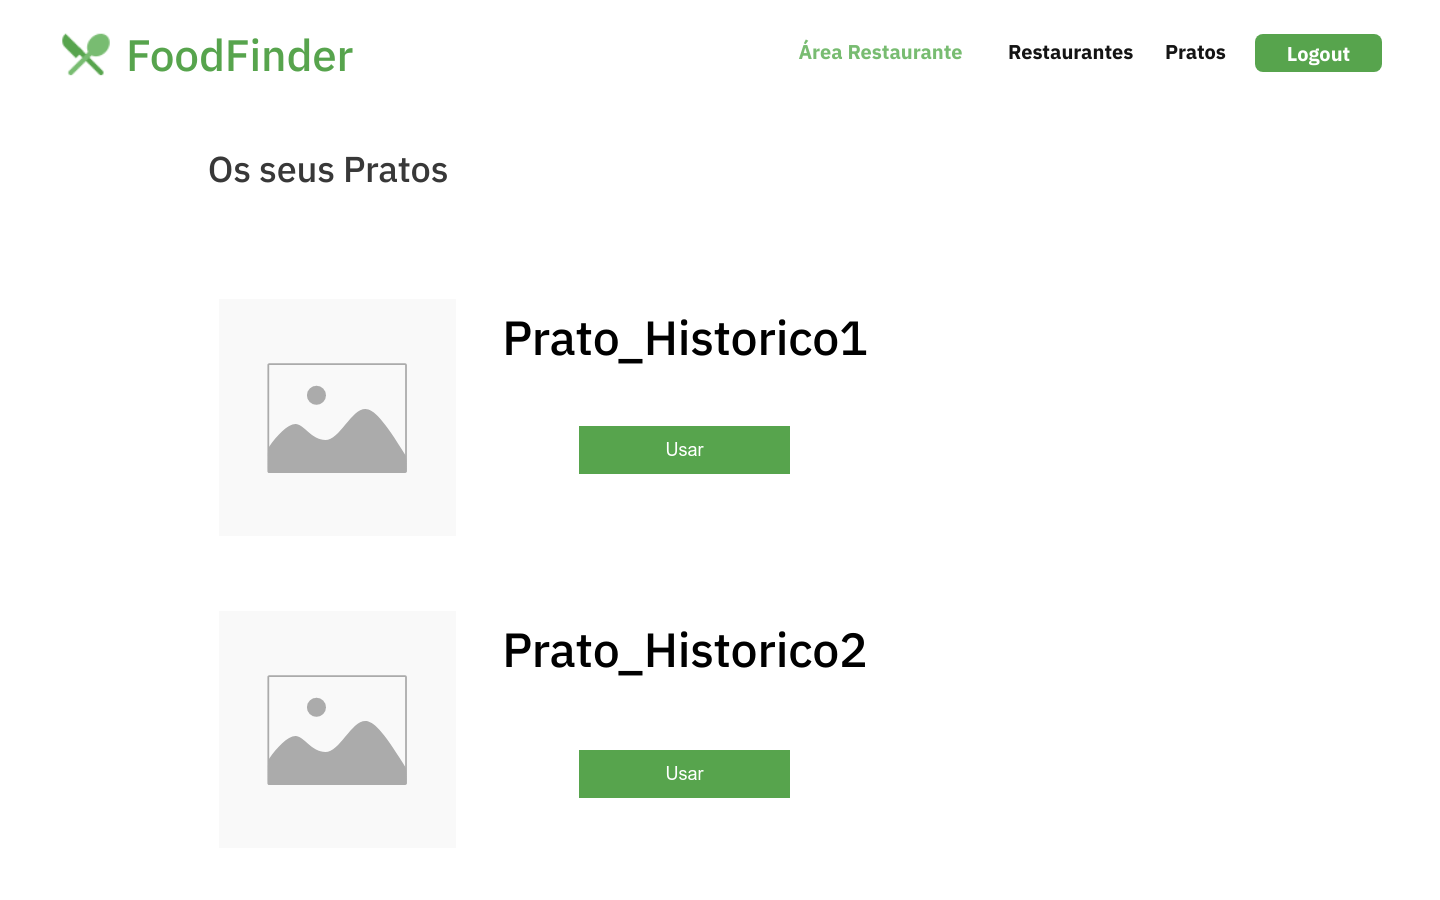
\includegraphics[scale=0.25]{10.1-Prato_Historico_restaurante}	
	\end{center}
	\caption{Interface que apresenta os pratos anteriores de um restaurante.}
	\end{figure} 
	
\section{Interfaces Específicas do Administrador}
	
	\begin{figure}[H]
	\begin{center}
	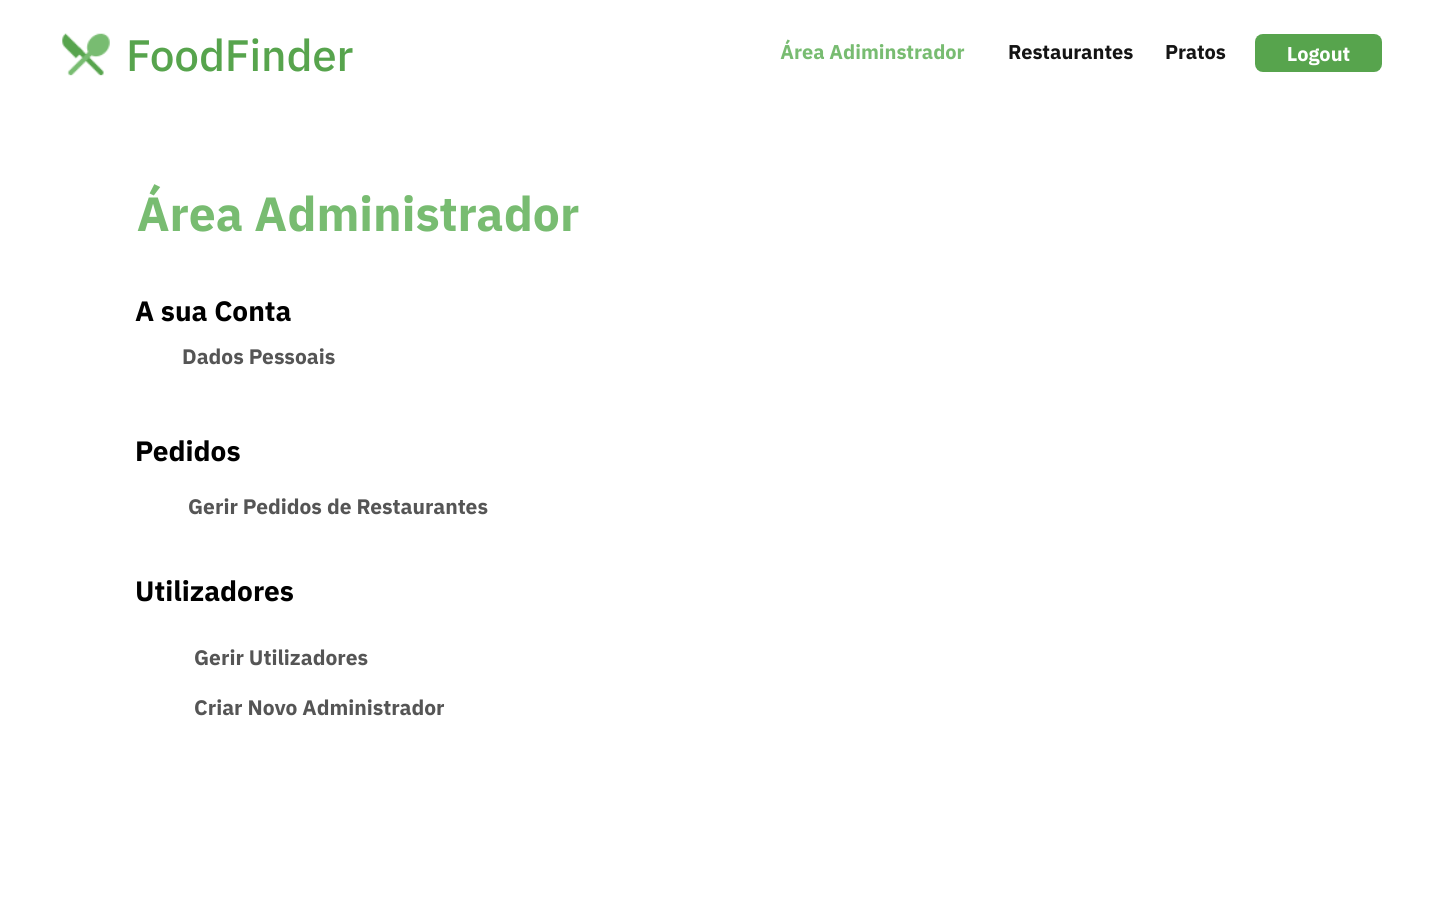
\includegraphics[scale=0.25]{12.1-Area_Administrador}	
	\end{center}
	\caption{Interface que apresenta o menu onde o administrador tem acesso às suas funcionalidades.}
	\end{figure} 
	
	\begin{figure}[H]
	\begin{center}
	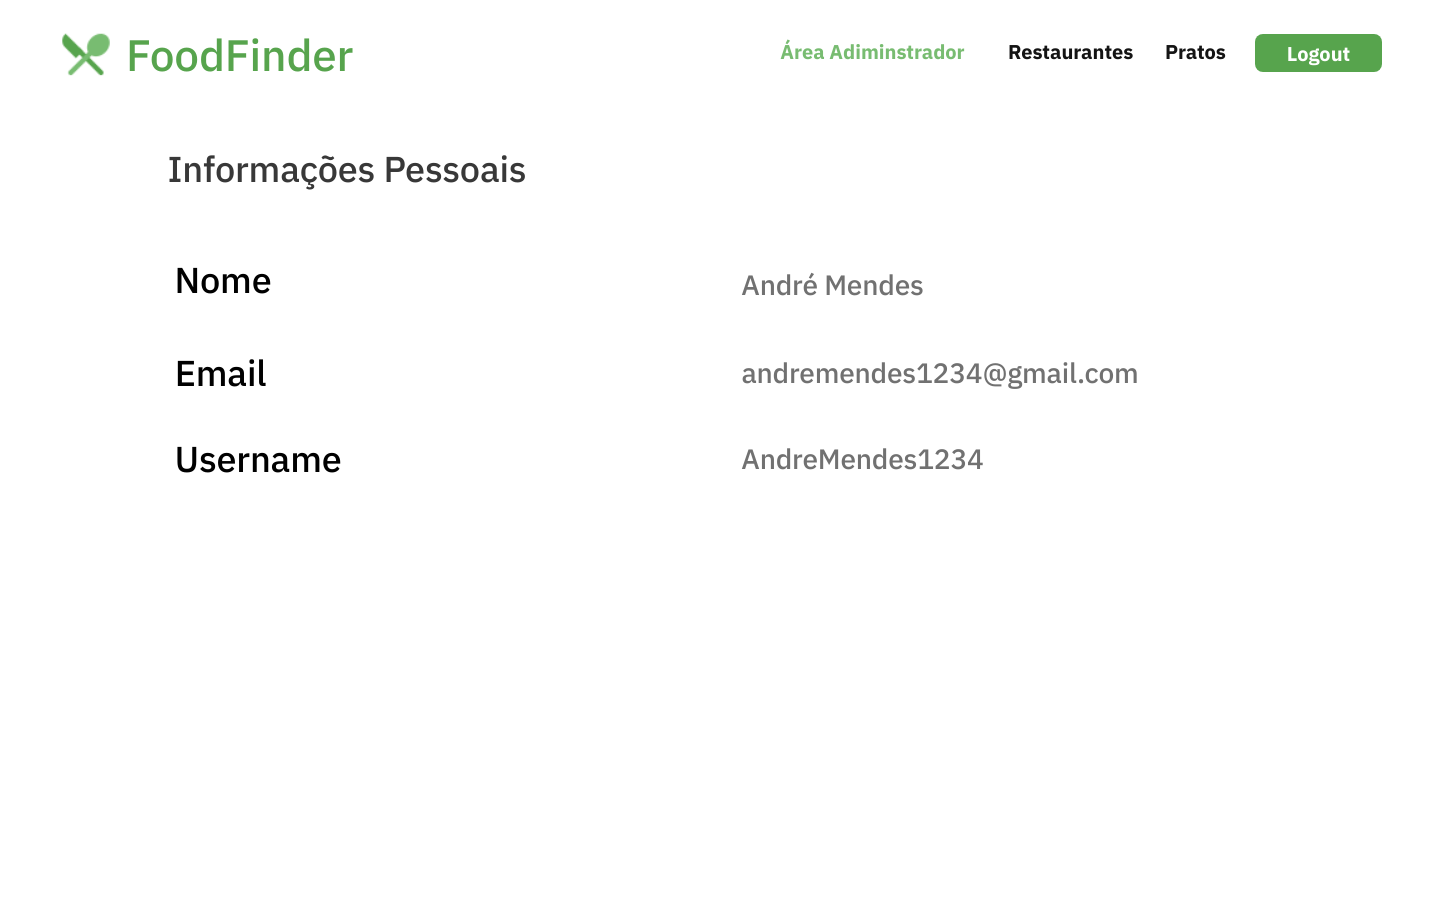
\includegraphics[scale=0.25]{13.1-Dados_Pessoais_Administrador}	
	\end{center}
	\caption{Interface que permite ao administrador consultar as suas próprias informações.}
	\end{figure} 
	
	\begin{figure}[H]
	\begin{center}
	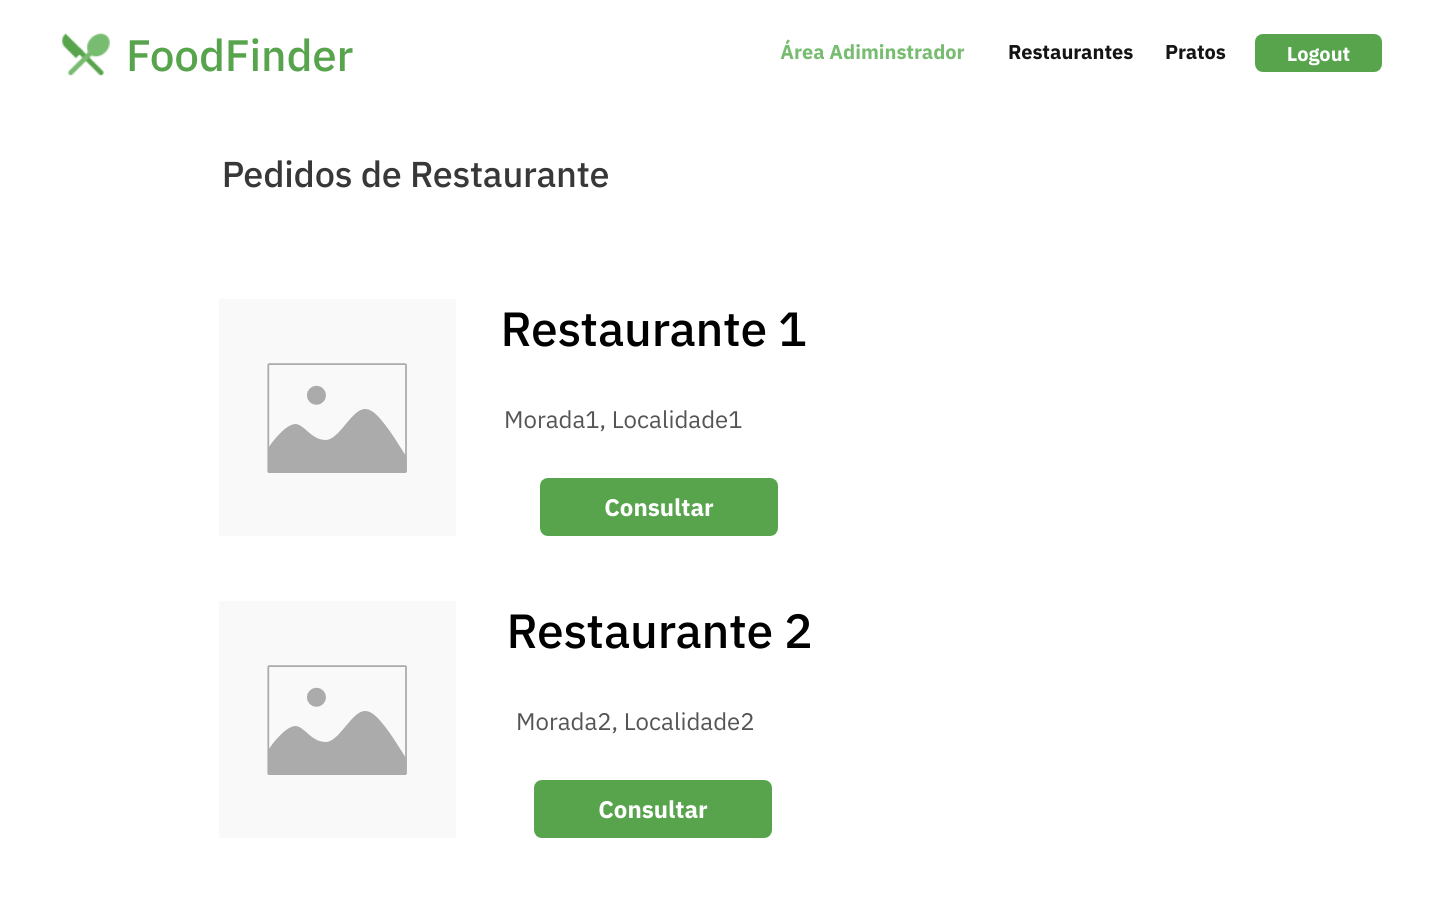
\includegraphics[scale=0.25]{14.1-Pedidos_Restaurante_Administrador}	
	\end{center}
	\caption{Interface que permite ao administrador verificar os novos pedidos de registo dos restaurantes.}
	\end{figure} 
	
	\begin{figure}[H]
	\begin{center}
	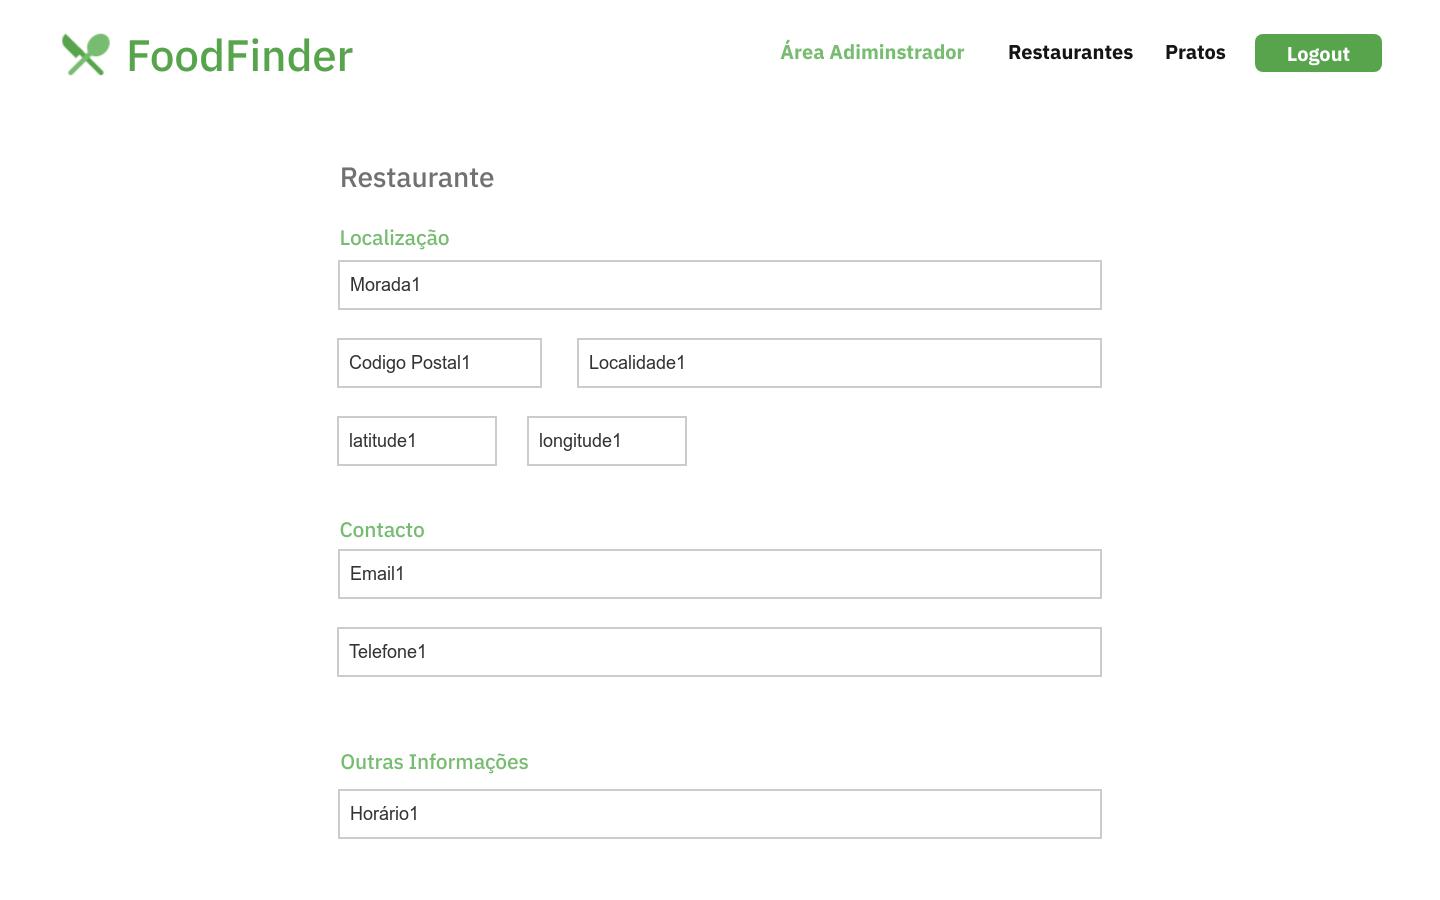
\includegraphics[scale=0.25]{15.1-Pedidos_Restaurante_Consultar_Administrador_1}	
	\end{center}
	\caption{Interface que permite ao administrador consultar a informação de um restaurante antes de aceitar ou recusar o seu pedido.}
	\end{figure} 
	
	
	\begin{figure}[H]
	\begin{center}
	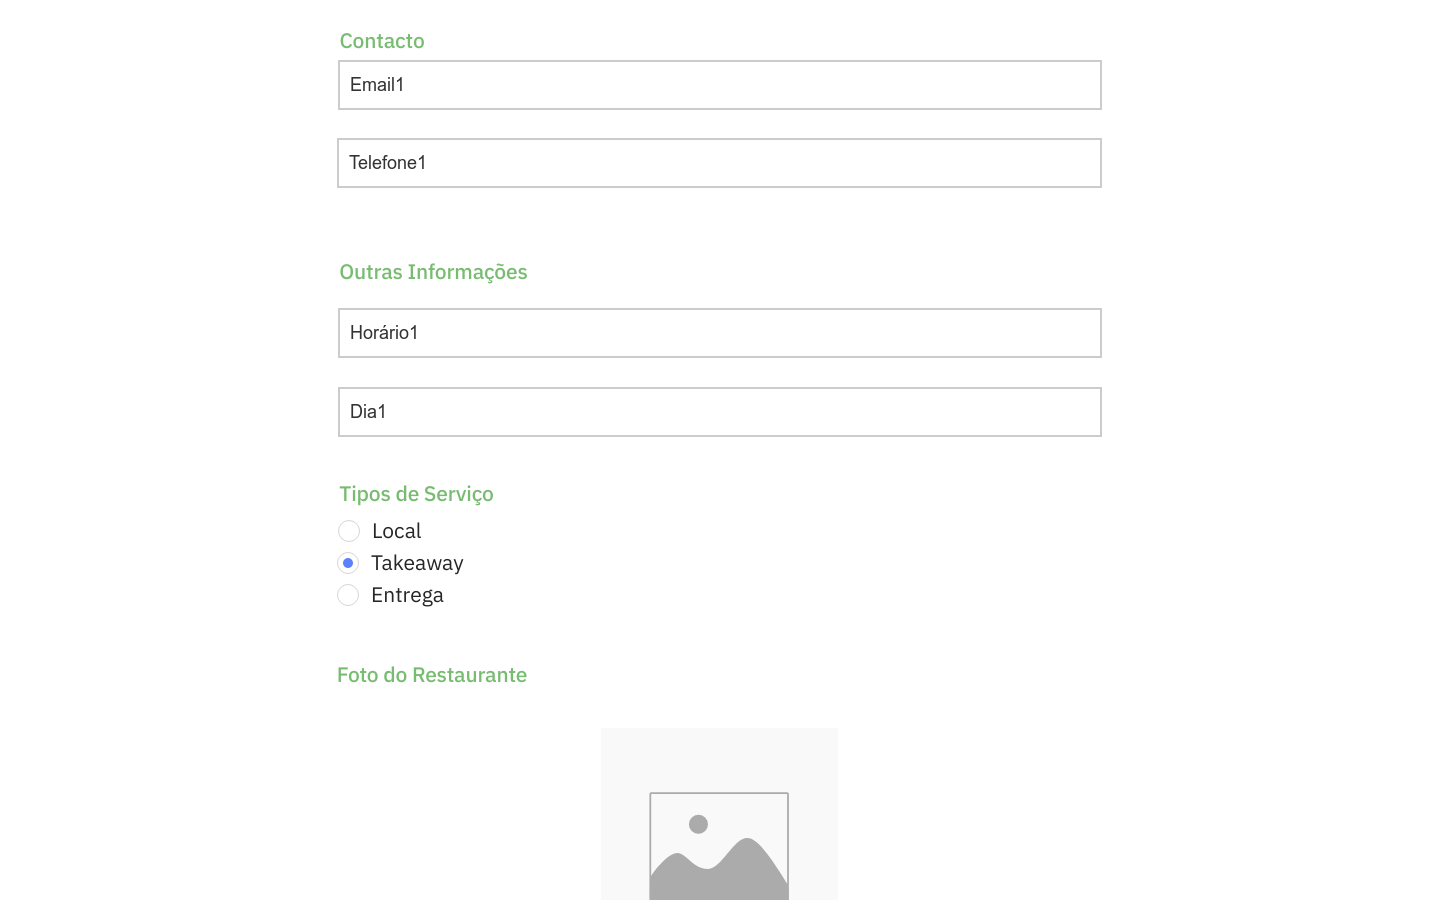
\includegraphics[scale=0.25]{16.1-Pedidos_Restaurante_Consultar_Administrador_2}	
	\end{center}
	\caption{Continuação da interface que permite ao administrador consultar a informação de um restaurante antes de aceitar ou recusar o seu pedido.}
	\end{figure} 
	
	\begin{figure}[H]
	\begin{center}
	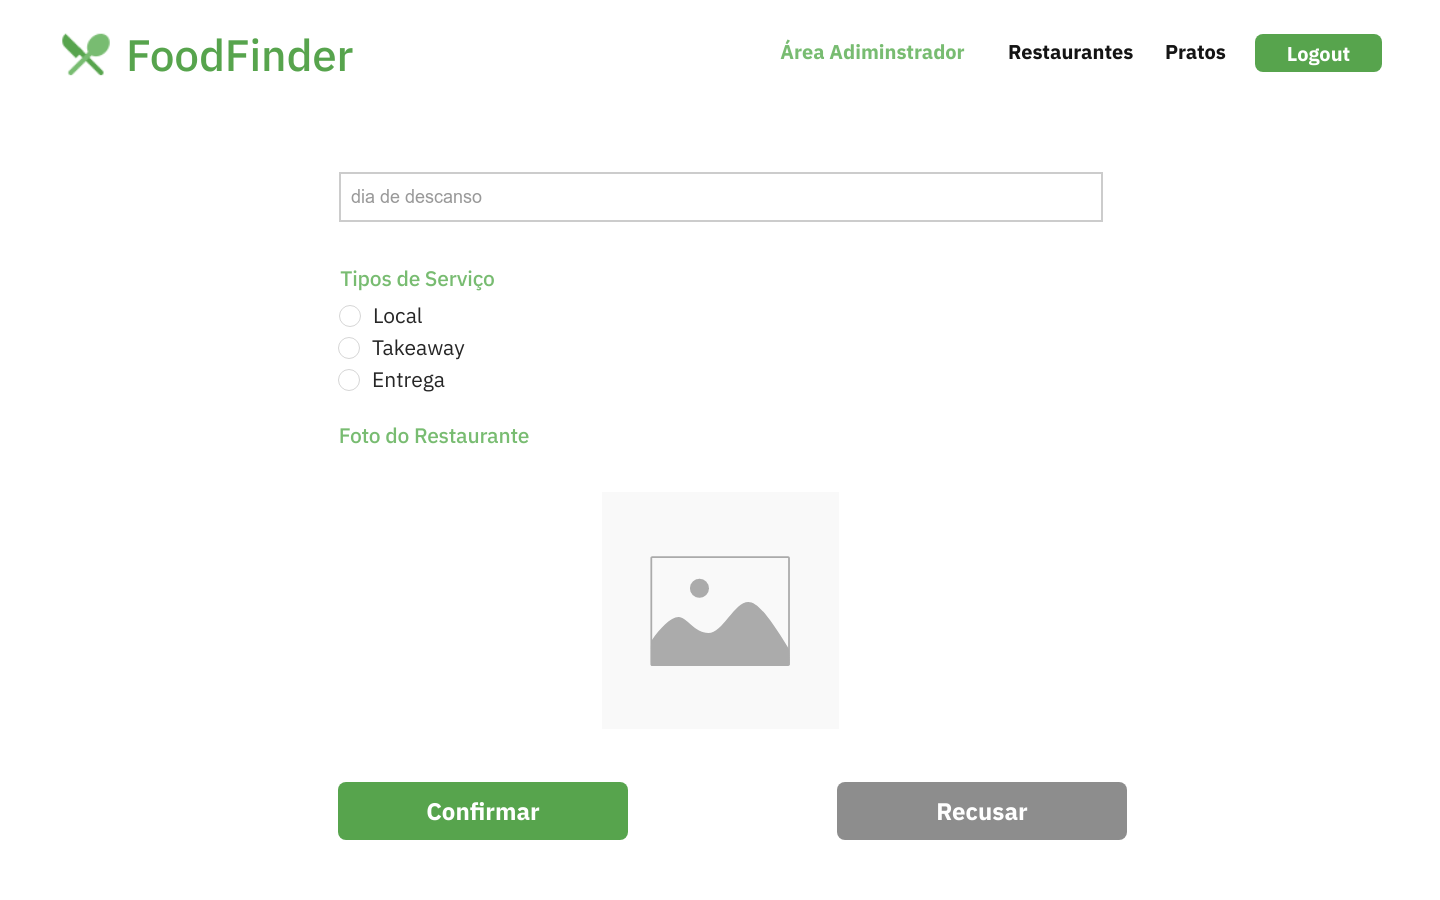
\includegraphics[scale=0.25]{17.1-Pedidos_Restaurante_Consultar_Administrador_3}	
	\end{center}
	\caption{Continuação da interface que permite ao administrador consultar a informação de um restaurante antes de aceitar ou recusar o seu pedido.}
	\end{figure} 
	
	\begin{figure}[H]
	\begin{center}
	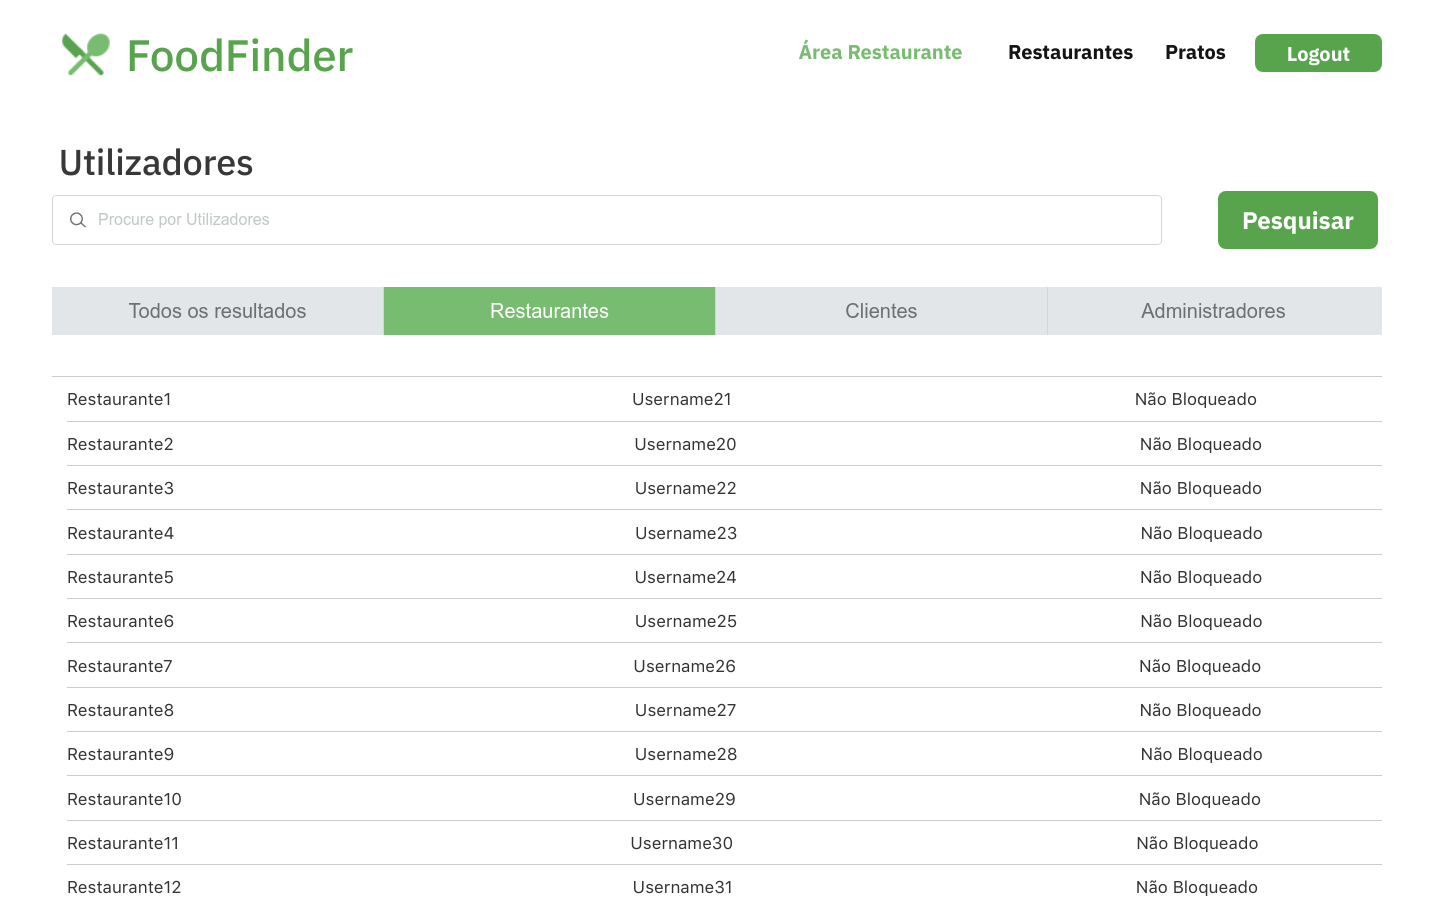
\includegraphics[scale=0.25]{18.1-Gerir_Utilizadores_Administrador_1}	
	\end{center}
	\caption{Interface que possibilita ao administrador consultar a listagem de todos os utilizadores registados no sistema.}
	\end{figure} 
	
	
	\begin{figure}[H]
	\begin{center}
	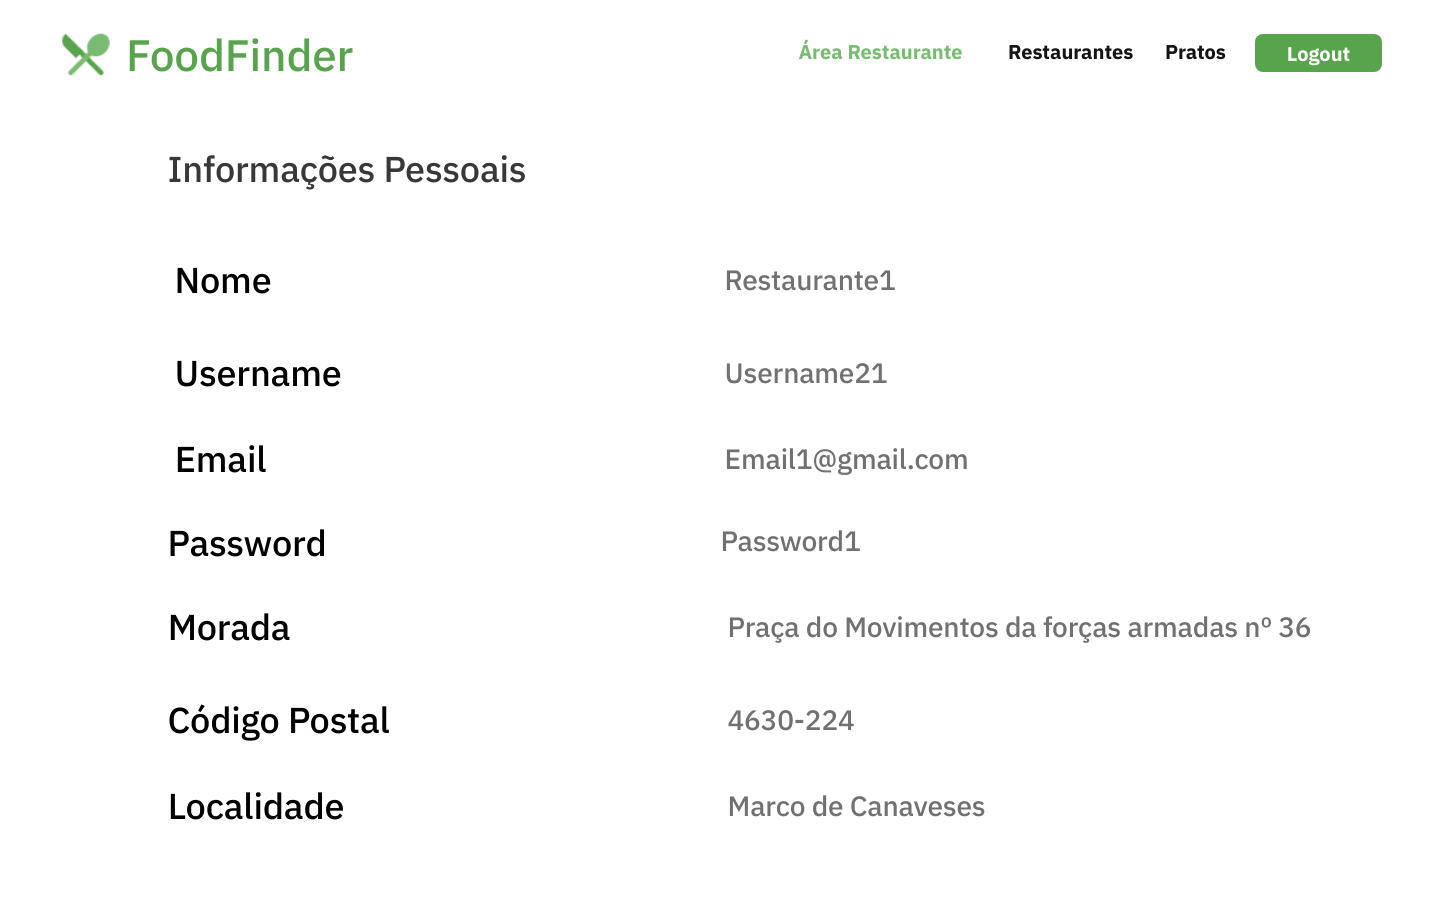
\includegraphics[scale=0.25]{20.1-Gerir_Utilizadores_restaurante_Administrador_1}	
	\end{center}
	\caption{Interface que permite ao administrador consultar a informação de um utilizador.}
	\end{figure} 
	
	
	\begin{figure}[H]
	\begin{center}
	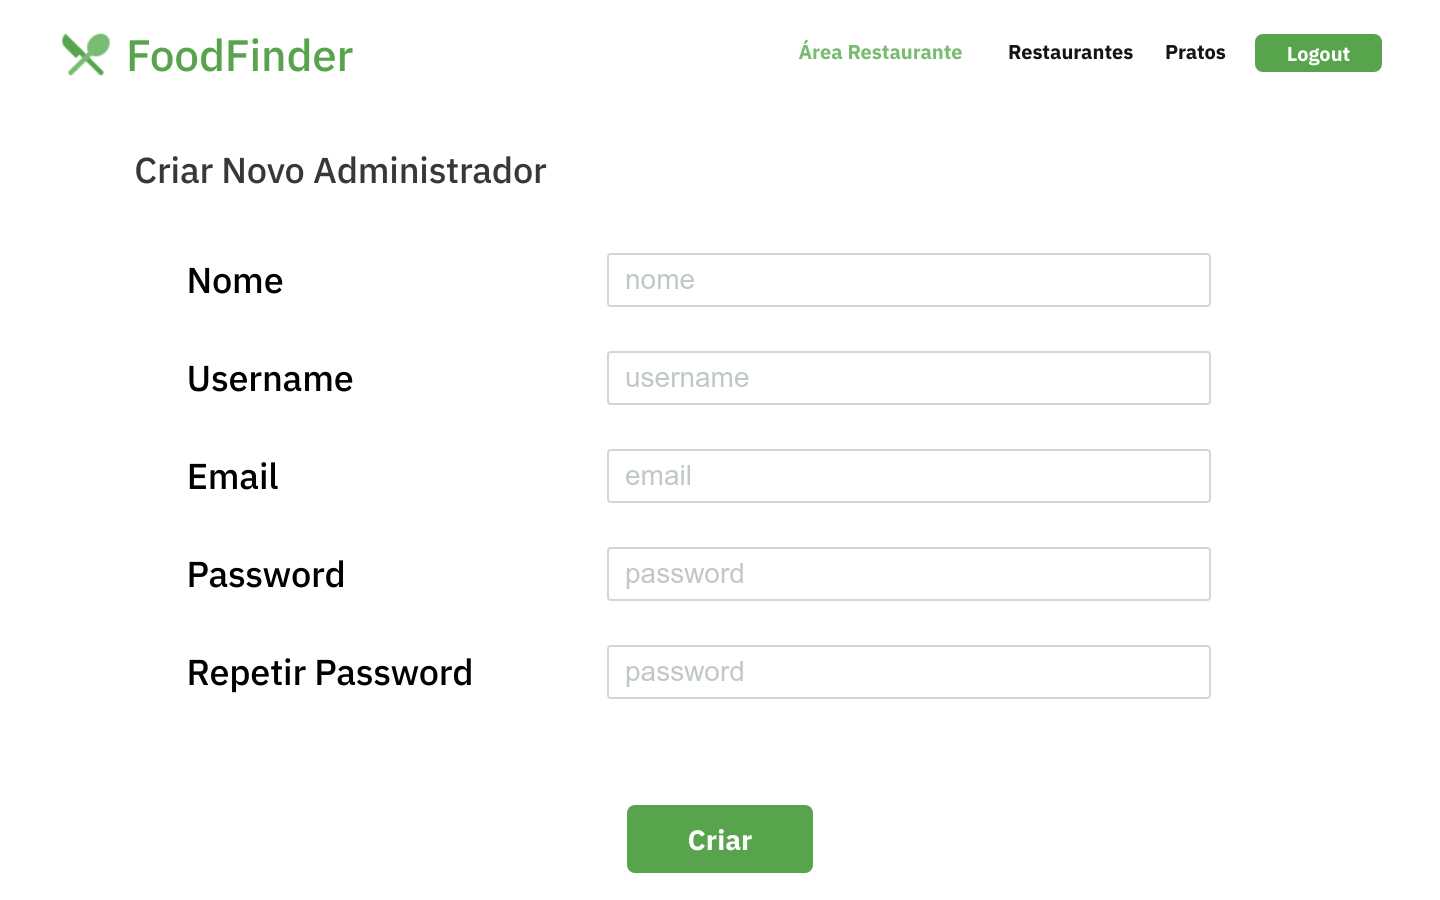
\includegraphics[scale=0.25]{22.1-Criar_Novo_Administrador}	
	\end{center}
	\caption{Interface que permite a um administrador criar outros administradores.}
	\end{figure} 
	
	

	

%--------------------------------------------------------------
\chapter{Conclusão}	

	A base de dados é um aspeto central da maioria dos sistemas de computação e, portanto, o seu cuidadoso planeamento e \textit{design} é essencial para o sucesso dos mesmos. Contudo, grande parte das aplicações dirigidas para o utilizador humano, requerem não só o bom funcionamento a nível lógico do sistema, como também uma \textit{interface} que permita ao utilizador fazer uso desse mesmo sistema de uma forma fluída e eficaz.  
	
	Neste estudo, procedemos ao mapeamento do modelo concetual para o modelo relacional da base de dados como a consequente implementação do modelo físico recorrendo à linguagem SQL. Assim, a base de dados encontra-se pronta para integrar o futuro sistema ainda a implementar.
	
	Da mesma maneira, desenhamos e apresentamos as \textit{mockups} da interface do sistema, permitindo, assim, fazermos uso delas como \textit{blueprints} para a fase da implementação da \textit{user interface} e da \textit{user experience}.
	
	Assim, podemos, até certo modo, dar por concluído o processo de \textit{planeamento} e \textit{design} dos aspetos mais fundamentais do nosso sistema. Contudo, temos que lembrar, tal como a história do desenvolvimento de \textit{software} nos mostrou, que este planeamento deverá ser feito de forma incremental e iterativa e, assim, admitimos que durante a própria execução e planeamento haverão momentos em que teremos que fazer um refinamento ou mesmo adição de novas funcionalidade e novas características. 
	
	

%--------------------------------------------------------	
\titleformat{\chapter}[display]
{\normalfont\bfseries}{}{0pt}{\Huge}
\chapter{Referências}

Captain, F. A. (2015). Six-step relacional database design: a step by step aproach to relational database desing and development. 

Jazayeri, M. (2007). Some trends in web application development. Conference Paper. 


%--------------------------------------------------------	
\newpage
\titleformat{\chapter}[display]
{\normalfont\bfseries}{}{0pt}{\Huge}
\chapter{Anexos}

\section{Anexo A - Código SQL para a Criação das Tabelas da Base de Dados} \label{anexoA}

\begin{lstlisting}
CREATE TABLE Bloqueado
(
	id BIGINT NOT NULL,
	motivo VARCHAR(50) NOT NULL,

	PRIMARY KEY (ID)
	);

CREATE TABLE Utilizador
(
	username VARCHAR(15) NOT NULL,
	email VARCHAR(50) NOT NULL,
	password VARCHAR(20) NOT NULL,
	nome VARCHAR(50) NOT NULL,
	registo_Confirmado BIT NOT NULL,
	bloqueado_ID BIGINT,

	PRIMARY KEY (Username),
	FOREIGN KEY (Bloqueado_ID) REFERENCES Bloqueado
);

CREATE TABLE Localizacao
(
	localizacao_id BIGINT NOT NULL,
	codigo_postal VARCHAR(15) NOT NULL,
	morada VARCHAR(50) NOT NULL,
	localidade VARCHAR(50) NOT NULL,
	gps_Latitude FLOAT NOT NULL,
	gps_Longitude FLOAT NOT NULL,

	CHECK(codigo_postal LIKE '[0-9][0-9][0-9][0-9]-[0-9][0-9][0-9]'),

	PRIMARY KEY (localizacao_id),
);

CREATE TABLE Restaurante
(
	restaurante_id VARCHAR(15) NOT NULL,
	contacto_email VARCHAR(25) NOT NULL,
	contacto_telefone BIGINT NOT NULL,
	horario_funcionamento VARCHAR(50) NOT NULL,
	dia_de_descanso VARCHAR (10) ,
	tipo_de_servico VARCHAR(50) NOT NULL,
	localizacao_id BIGINT NOT NULL,
	rating INT NOT NULL,
	descricao VARCHAR(300) NOT NULL,
	
	CHECK(contacto_telefone > 0),

	PRIMARY KEY (restaurante_id),
	FOREIGN KEY (restaurante_id) REFERENCES Utilizador(username),
	FOREIGN KEY (localizacao_id) REFERENCES Localizacao(localizacao_id),
);

CREATE TABLE Cliente
(
	cliente_id VARCHAR(15) NOT NULL,

	PRIMARY KEY (cliente_id),
	FOREIGN KEY (cliente_id) REFERENCES Utilizador(username)
);

CREATE TABLE Administrador
(
	administrador_id VARCHAR(15) NOT NULL,

	PRIMARY KEY (administrador_id),
	FOREIGN KEY (administrador_id) REFERENCES Utilizador(username)
);

CREATE TABLE Comentario_Restaurante
(
	comentario_id BIGINT NOT NULL,
	data_comentario DATE NOT NULL,
	restaurante_id VARCHAR(15) NOT NULL,
	cliente_id VARCHAR(15) NOT NULL,
	corpo VARCHAR(300) NOT NULL,

	PRIMARY KEY (comentario_id),
	FOREIGN KEY (restaurante_id) REFERENCES Restaurante(restaurante_id),
	FOREIGN KEY (cliente_id) REFERENCES Cliente(cliente_id)
);


CREATE TABLE Prato_do_Dia
(
	prato_id BIGINT NOT NULL,
	descricao VARCHAR(300) NOT NULL,
	tipo VARCHAR(15) NOT NULL,

	PRIMARY KEY (prato_id)
);


CREATE TABLE Adicionar_Prato_do_Dia
(
	restaurante_id VARCHAR(15) NOT NULL,
	prato_id BIGINT NOT NULL,
	data_prato DATE NOT NULL,
	preco FLOAT NOT NULL,
	destacado BIT NOT NULL,

	PRIMARY KEY (prato_id, restaurante_id, data_prato),
	FOREIGN KEY (restaurante_id) REFERENCES Restaurante(restaurante_id),
	FOREIGN KEY (prato_id) REFERENCES Prato_do_Dia
);

CREATE TABLE Favoritar_Restaurante
(
	restaurante_id VARCHAR(15) NOT NULL,
	cliente_id VARCHAR(15) NOT NULL,

	PRIMARY KEY (restaurante_id, cliente_id),
	FOREIGN KEY (restaurante_id) REFERENCES Restaurante(restaurante_id),
	FOREIGN KEY (cliente_id) REFERENCES Cliente(cliente_id),
);

CREATE TABLE Favoritar_Prato_do_Dia
(
	prato_id BIGINT NOT NULL,
	cliente_id VARCHAR(15) NOT NULL,

	PRIMARY KEY (prato_id, cliente_id),
	FOREIGN KEY (prato_id) REFERENCES Prato_do_Dia(prato_id),
	FOREIGN KEY (cliente_id) REFERENCES Cliente(cliente_id),
);

\end{lstlisting}

	
\end{document}